%% 
%% Copyright 2019-2024 Elsevier Ltd
%% 
%% Version 2.4
%% 
%% This file is part of the 'CAS Bundle'.
%% --------------------------------------
%% 
%% It may be distributed under the conditions of the LaTeX Project Public
%% License, either version 1.2 of this license or (at your option) any
%% later version.  The latest version of this license is in
%%    http://www.latex-project.org/lppl.txt
%% and version 1.2 or later is part of all distributions of LaTeX
%% version 1999/12/01 or later.
%% 
%% The list of all files belonging to the 'CAS Bundle' is
%% given in the file `manifest.txt'.
%% 
%% Template article for cas-sc documentclass for 
%% single column output.

% \documentclass[a4paper,fleqn,longmktitle]{cas-sc}
\documentclass[a4paper,10pt]{cas-sc}%,fleqn

\usepackage[numbers]{natbib}
% \usepackage[authoryear]{natbib}
% \usepackage[authoryear,longnamesfirst]{natbib}
\usepackage{bm}  
\usepackage{float} % 导入 float 宏包
% \usepackage{array}  % 确保引入该宏包
\usepackage{tabularx}
\usepackage{xcolor}
\definecolor{revisionred}{RGB}{190,0,0}
\newcommand{\rev}[1]{\textcolor{revisionred}{#1}}
\newenvironment{revision}{\color{revisionred}}{}
\AtBeginEnvironment{Abstract}{\color{revisionred}}
% \usepackage{times}
% \renewcommand{\familydefault}{\rmdefault} % 将默认字体设置为 Times New Roman


% \doublespacing


%%%Author macros
\def\tsc#1{\csdef{#1}{\textsc{\lowercase{#1}}\xspace}}
\tsc{WGM}
\tsc{QE}
\tsc{EP}
\tsc{PMS}
\tsc{BEC}
\tsc{DE}
%%%

\begin{document}
\let\WriteBookmarks\relax
\def\floatpagepagefraction{1}
\def\textpagefraction{.001}
\shorttitle{}
\shortauthors{Anonymous Authors} % <--- ANONYMIZED
\let\printorcid\relax % Do not print ORCID.



\title [mode = title]{Correct-and-then-Detect: Adaptive Fault Detection through Data-driven Digital Twins and Transfer Learning}
% \tnotemark[1]

% \tnotetext[1]{The first author would like to acknowledge the support of Program of China Scholarship Council (202307090014).}



\begin{abstract}
	\rev{In a digital twin-based fault detection framework, it is essential to have a reliable and robust digital twin to generate reference values representing nominal behaviors. Traditional digital twin modelling approaches require deep understanding of functioning principles and failure mechanisms of the system, which are not always available in practice. Furthermore, as systems operate, maintaining an accurate digital twin becomes challenging as system's behavior tends to deviate from its nominal cases due to various factors like aging, uncertainty and sim-to-real gaps. To address these issues and better support predictive maintenance, this paper proposes an integrated framework for data-driven digital twin modeling and fault detection. First, we develop a design-of-experiment-based approach to generate training data that can efficiently cover the potential task space. The generated training data are then used to train a data-driven digital twin, \emph{i.e.,} a deep learning model that predicts system performances at a given time instant given observed covariates from a time window prior to it. Next, we develop a new adaptive fault detection method based on the developed data-driven digital twin. The algorithm works in an adaptive manner: first, the reference values generated by the digital twin is screened and corrected to remove potential contaminations from faulty signals in the context window. Then, the corrected reference values are used in a residual-based framework for fault detection. Finally, a transfer learning mechanism is applied in the developed framework to make sure the performance of the data-driven digital twin and fault detection methods remain robust under system evolution and cross-domain distribution shifts. Real experiments are conducted on two real robots. The results confirm that the data-driven digital twin model accurately captures the actual behavior of the physical entity and that the developed adaptive fault detection methods provide more accurate and robust results compared to traditional methods.}
\end{abstract}

\begin{keywords}
	Data-driven digital twin,\sep predictive maintenance, \sep fault detection, \sep domain adaptation, \sep transfer learning, \sep robot arm
\end{keywords}

\maketitle

%
% Introduction
%
\section{Introduction}

% With the development of industrial systems toward higher complexity, greater autonomy, and long-term continuous operation, achieving reliable condition monitoring and fault detection during system operation has become one of the core challenges in intelligent maintenance and predictive maintenance\cite{ENGBERS2025964, garcia2025condition, wu2025data}. 
Complex industrial systems like industrial robots typically operate under complex and strongly nonlinear environments. Their operational behavior evolves over time because of aging, parameter drift, and environmental variations \citep{QIAO201851, lei2025condition}. Reliable condition-monitoring and fault detection for such systems are therefore important but challenging issues \citep{SABRY2024102397}. Traditionally, fault detection methods for complex industrial systems mainly rely on statistical analyses of measured data and residuals \citep{SABRY2024102397}. Typical methods in this category include signal processing-based approaches, rule-based systems, and model-based methods \citep{SABRY2024102397, 9529495}. A detailed review of such methods is presented in Sect. ~\ref{sec:2.1}. As can be seen in Sect. ~\ref{sec:2.1}, a major limitation of these traditional methods is that they require handcrafted features or accurate mathematical models, which are often unavailable for complex systems operating under frequently-changing operating conditions.

As an alternative to the statistical analyses of measured data and residuals, data-driven fault detection methods become increasingly common as they do not require handcrafted features or explicit system models \citep{SABRY2024102397, 9529495}. Instead, they learn fault-discrimination patterns directly from historical data using machine learning or deep learning models \citep{SABRY2024102397, 9529495} (see Sect. \ref{sec:2.1} for a detailed review). As shown in Sect. \ref{sec:2.1}, while performing generally well on high-dimensional nonlinear systems, the machine learning/deep learning-based methods generally require large amounts of labeled fault data for training. In industrial systems, fault events are often rare and uncontrollable, which limits practical deployment.

To reduce dependence on labeled fault data, digital twin technology has been introduced into fault detection \citep{hosamo2022review, darvishi2020sensor}. In these methods, a digital twin is developed to represent nominal system behavior and supplies reference values for measured data. Faults are then detected from residuals between measurements and their references. As discussed in Sect. ~\ref{sect:2.3}, existing digital twin faces a critical challenge: developing high-fidelity physics-based or simulation-based digital twins relies on in-depth domain knowledge and precise parameter calibration, making them difficult to build, especially for complex systems under long-term operation \citep{HU2025102963, YOU20221471}.

In recent years, data-driven digital twins have attracted increasing attention as an alternative paradigm that integrates data-driven modeling with virtual--physical mapping \citep{teng2021recent, friederich2022framework, 10477658, hui2022digital}. The core idea is to learn the nominal behavior of the system from healthy operational data and to formulate fault detection as the identification of deviations from nominal behavior \citep{Michau_2019}. Compared with direct fault classification approaches, this paradigm offers clear advantages in terms of data availability and engineering feasibility \citep{ZHONG2023e14534}. \rev{The nominal predictor is not itself the fault detector: it supplies an operating-condition-dependent reference from which a residual is constructed, and the residual is subsequently used to support fault detection.} However, as analyzed in detail in Sect. \ref{sect:2.3}, existing data-driven digital twin methods still face three challenges: (1) most existing data-driven digital twin models lack systematic experimental design to ensure sufficient coverage of the operational space in the training phase, which limits their accuracy and generalization capability; (2) the developed digital twins easily become outdated when system behavior changes during operation; (3) the reference values predicted by the digital twins can be contaminated by fault-affected inputs because most data-driven digital twins use a rolling window to make predictions.

\rev{To address these limitations, this paper develops a digital-twin-driven fault detection framework that is able to (1) efficiently design training data generation process to ensure the coverage of the generated training data; (2) remains robust under system evolution and cross-domain distribution shifts ; and (3) remains insensitive to the data contamination brought by faulty signals. The main contributions are:}
\begin{itemize}
	\color{revisionred}
	\item A DoE-guided data acquisition and rolling-horizon modeling procedure is established. Through Halton sampling, the generated training data fully cover a bounded task-configuration envelope, making sure the trained model fully learns the typical application scenarios of the target system;
	\item A transfer learning-based framework is developed to update the developed data-driven digital twins under system evolution and cross-domain distribution shifts.
	\item A threshold-triggered contamination-suppression mechanism, named Prediction-based Recursive Observation Feedback (PROF), is introduced to avoid data contamination caused by including faulty signals into the context window of the data-driven digital twin. 
	\item An open dataset from two real robots is released to validate the developed data-driven digital twin modeling and fault detection framework.
\end{itemize}
\rev{It should be noted that the main contribution here is the integrated data-driven fault detection framework, including nominal behavior modeling, transfer-learning-based digital twin updating, and PROF-enhanced residual fault detection, rather than the performance of its individual building blocks like prediction accuracy of the digital twin.}

The remainder of this paper is organized as follows.
Section~\ref{sec:2} reviews related work on fault detection and digital twin modeling.
Section~\ref{sec:3} presents the proposed data-driven digital twin framework with transfer learning.
Section~\ref{sec:4} introduces the residual-based fault detection method and the PROF mechanism.
Section~\ref{sec:5} describes the experimental setup.
Section~\ref{sec:6} reports and analyzes the experimental results.
Section~\ref{sec:7} concludes the paper.

\section{Related work}\label{sec:2}

In this section, we review the related works with a focus on their limitations. In Sect. \ref{sec:2.1}, we review traditional approaches for \rev{fault detection}. Recent works on digital twin-based fault detection are discussed in Sect. \ref{sect:2.2}. In Sect. \ref{sect:2.3}, \rev{we} discuss data-driven digital twin modeling.

\subsection{Traditional fault detection methods}\label{sec:2.1}

% Including traditional, and data-driven. You end with a summary of gaps: Lack of labeled failure data
According to \citep{9529495, leite2024fault}, traditional fault detection methods can be classified into model-based, signal-based, and data-driven approaches. Model-based techniques use explicit mathematical representations of nominal system dynamics to detect deviations between observed and predicted behavior \citep{ISERMANN1997709, marzat2012model}. For example, observer-based residual generation methods construct state estimators such as Kalman filters and Luenberger observers to compare measured outputs with model predictions, where residual signals are monitored for significant deviations indicating faults. Prior work has applied such observers for actuator fault diagnosis in benchmark systems, demonstrating their ability to detect anomalies by thresholding estimation residuals \citep{Zemali2023}. Fuzzy model-based observers have also been designed for detecting sensor faults in chemical process systems, where multiple observer structures are evaluated based on their residual generation performance \citep{BALLESTEROSMONCADA2015325}. While effective when accurate models exist, they struggle in complex systems due to the difficulty of capturing nonlinear interactions and detailed normal/fault behaviors, especially for components like actuators and sensors \citep{JUNG2019285}.

Signal-based methods extract features from raw measurements, such as spectral or statistical characteristics, and compare them to reference profiles \citep{aiorduachioaie2024comparative, wu2019survey}. For example, time--frequency spectral amplitude modulation methods extract characteristic fault features from vibration signals by combining short-time Fourier transform with weighted spectral amplitude analysis, enabling effective detection of bearing faults under noisy conditions \citep{JIANG2023109832}. Similarly, advanced machine health monitoring approaches leverage time--frequency feature extraction techniques to identify modulation patterns induced by transmission element faults, such as amplitude and frequency modulations in rotating machinery vibration signals \citep{ZHOU2023110489}. These approaches avoid reliance on explicit system models but depend on carefully designed feature extraction and thresholding, which are difficult to generalize across varying operating conditions or high-dimensional industrial data. 

Data-driven methods leverage machine learning to infer fault patterns directly from data without explicit physical models. They can automatically capture complex temporal and spatial correlations using approaches such as support vector machines or neural networks \citep{sahu2024data, dai2013model, chen2023review, calabrese2022data}. For example, data-driven fault diagnosis methods have been widely applied in rotating machinery, where convolutional neural networks are trained to classify fault types directly from raw vibration signals without explicit feature design \citep{SOUZA2021107060}. Deep learning models have also been used to detect and distinguish incipient and compound faults in industrial systems by learning complex representations from multi-sensor time-series data, often outperforming traditional machine learning classifiers on benchmark datasets \citep{neupane2025data}. These approaches avoid reliance on explicit physical models and can automatically capture intricate temporal and spatial correlations in the data. However, most data-driven methods require large quantities of labeled fault data for supervised training. In real industrial environments, fault events are often rare to observe. Obtaining enough labeled failure data is often difficult considering the constraints of costs and safety \citep{neupane2025data, ramirez2023semi, saeed2025deep}.


\subsection{Digital twin-based fault detection}\label{sect:2.2}

% Review some existing works. Start by physics/simulation-based DT. Gaps: Difficult to get the DT model like this. Also, mention that the rolling window will be contaminated by the failure data (window contamination problem).


Digital twin technology provides a virtual replica of a physical system that can be used for monitoring, simulation, and fault diagnosis \citep{javaid2023digital,ZHONG2023e14534}. In fault detection applications, digital twins are often constructed using physics-based or simulation models that emulate the detailed behavior of the physical entity. These high-fidelity models can generate synthetic data under various operating conditions, support predictive analysis, and enable the exploration of fault scenarios that are difficult to observe directly on the physical system \citep{lopes2024synthetic, van2022predictive}. For example, digital twin models of electric machines have been used to simulate motor dynamics and extract fault-relevant features for diagnostic tasks \citep{hu2025research}. Similarly, physics-based digital twin models have been applied to gearbox fault diagnosis, where multi-physical simulations generate virtual vibration data for training diagnostic models \citep{xia2023novel}. Recent work has attempted to integrate virtual and physical data for fault detection and diagnosis. Through physical-virtual data fusion or hybrid modeling, the quality of synthetic fault data and diagnosis performance can be improved \citep{xia2023novel,xia2024digital}.

While physics/simulation-based digital twins offer substantial potential for fault detection, they also face significant challenges. Constructing detailed physics models that faithfully represent all relevant behaviors of complex systems is resource intensive, requiring comprehensive domain knowledge and extensive calibration. In addition, such models often depend on simplified assumptions or idealized conditions that limit their ability to capture real-world variability in operational environments, sensor noise, and degradation processes. These limitations make it difficult to scale physics-based twin models to diverse systems or to maintain them over long operating life cycles \citep{van2022predictive, ZHONG2023e14534}. Moreover, discrepancies between simulated and real system behavior can degrade diagnostic accuracy when models are applied in practice.


\subsection{Data-driven digital twin modeling}\label{sect:2.3}

% Review some work that use data-driven approach to develop digital twin. Gaps: No design of experiment is considered -> Cannot ensure teh coverage and efficiency of the training data. Gaps: No transfer learning -> Hard to generalize. 

As an alternative to physics-based digital-twin modeling, data-driven approaches have been used increasingly. These approaches train statistical or machine-learning models on sensor data collected under normal conditions, without requiring detailed physical or simulation models \citep{kreuzer2024artificial,nele2024towards, khan2025data}. Data-driven twins capture system behavior directly from data streams and have been applied to real-time monitoring, anomaly detection, and fault diagnosis. For example, streaming sensor data have been used to update machine-monitoring models and identify deviations indicative of faults \citep{cheruku2025data}. Long short-term memory (LSTM) networks have also been embedded in digital twins for fault diagnosis of electro-hydrostatic actuators, demonstrating that learned representations can support detection without explicit physical models \citep{rodriguez2024development}.


Despite these advances, current data-driven digital twin research exhibits notable limitations as well. First, most existing studies collect training data from available operational traces without systematic design of experiments (DoE) to ensure coverage of relevant system behaviors across different operating conditions. Without proper experiment designs, the learned models may lack sufficient diversity to generalize beyond the scenarios represented in the training set. Second, although some works integrate machine learning within digital twin structures, few explicitly address transfer learning or domain adaptation to enhance model generalization when the operating domain shifts or when the digital twin is deployed on new systems or environments. As a result, data-driven twins trained on one dataset may perform poorly when applied to unseen conditions.


\section{Data-driven digital twin modeling with design-of-experiment and transfer learning}\label{sec:3}

In this section, we develop a data-driven digital twin framework for nominal behavior modeling.
Section~\ref{sec:3.1} formalizes the problem setting.
Section~\ref{sec:3.2} constructs the rolling-horizon predictive digital twin through design-of-experiments--based data acquisition, temporal sample construction, and sequence model learning.
Section~\ref{sec:3.3} presents a transfer learning strategy for adaptive updating under system evolution.

\subsection{Problem definitions}\label{sec:3.1}

We consider a physical system that generates a multivariate response that is observable at time instants $t_1, t_2,...,t_n$. The objective of a data-driven digital twin is to predict the system response by mapping historical observations to the future evolution of a quantity of interest over a finite prediction horizon.
To formally define the problem, let us assume that we observe the system's response $\mathcal{Y}$ and covariate $\mathcal{X}$ at fixed instants. Let $w$ denote the size of a sliding window, inside which the covariates are used to build the data-driven digital twin. Conceptually, our task is to build a predictive operator mapping from the observation history to the predicted performance at a future instant. Let $\mathcal{X}^{\ast}$ denote the space of finite observation histories and let $\mathcal{Y}^H$ denote the space of target trajectories over a horizon of length $H$. At each time step $t$, the prediction task is described by a distribution-conditioned operator
\begin{equation}
	\label{eq:operator}
	\mathcal{T}_{\mathbb{P}_t} : \mathcal{X}^{\ast} \rightarrow \mathcal{Y}^H,
\end{equation}
where $\mathbb{P}_t$ denotes the data distribution governing the system observations at time $t$. As the system operates, the data-driven digital twin in ~\eqref{eq:operator} can be applied sequentially to predict the system performance online. When new data become available, the context window $w$ moves forward in a rolling-horizon manner to reflect system status changes. In Sect. \ref{sec:3.2}, we first present a new DoE-based framework to develop the digital twin model in Eq. ~\eqref{eq:operator}.

In long-term operation, the underlying data distribution $\mathbb{P}_t$ may evolve due to changes in operating conditions, system dynamics, or environmental factors. Consequently, the predictive operator is not assumed to be static, but may evolve over time in response to distributional changes. This evolution is abstractly expressed as
\begin{equation}
	\label{eq:evolution}
	\mathcal{T}_{\mathbb{P}_{t+1}}
	=
	\mathcal{U}\!\left(\mathcal{T}_{\mathbb{P}_t},\, \mathbb{P}_{t+1}\right),
\end{equation}
where $\mathcal{U}(\cdot)$ denotes a generic update mechanism driven by newly observed data. As the system operates and a distribution shift arises, the performance of a fixed data-driven digital twin can deteriorate. To address this issue, Sect.~\ref{sec:3.3} introduces a transfer-learning-based updating approach.

\subsection{Data-driven digital twin modeling through rolling-horizon prediction}\label{sec:3.2}

This section presents the developed data-driven framework for digital twin modeling.
Figure~\ref{fig:framework_overview} provides an overview of the proposed framework.
The framework consists of three successive phases.
Phase I establishes a principled experimental design and data acquisition process to collect representative nominal operational data (Section~\ref{sec3.2.1}).
\rev{Phase II constructs a rolling-horizon data-driven digital twin by organizing multivariate measurements into finite observation-history vectors, forming temporally structured input--output samples, and training a predictive model for short-horizon forecasting (Sections~\ref{sec3.2.2} and~\ref{sec:3.2.3}).}
This predictive model serves as the core representation of the digital twin for online prediction and residual computation. In Phase III, online monitoring data are used to update the developed digital twin through transfer learning, as discussed in Sect.~\ref{sec:3.3}.

\begin{figure}
	\centering
	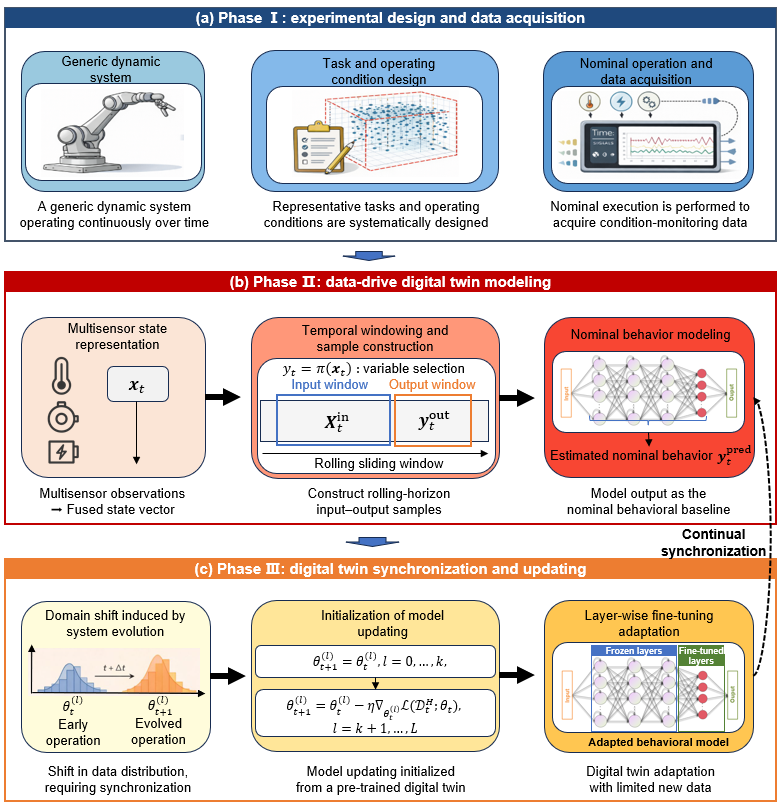
\includegraphics[width=.95\textwidth]{figs/framework_overview.png}
	\caption{Overview of the proposed data-driven digital twin framework.
		Phase~I establishes a principled experimental design and data acquisition layer, in which representative operating scenarios are systematically designed and executed to collect nominal condition-monitoring data from a generic dynamic system.
		Phase~II constructs a data-driven digital twin by transforming multisensor observations into rolling-horizon input--output samples and learning a predictive model that serves as a nominal behavioral baseline.
		Phase~III addresses long-term system evolution by continuously synchronizing and updating the digital twin in response to distributional shifts, enabling adaptive prediction under changing operating conditions.}
	\label{fig:framework_overview}
\end{figure}

\subsubsection{Data acquisition via design of experiments}\label{sec3.2.1}

\rev{
	The purpose of this phase is to design experiments and collect representative training data so that the training data fill as much as possible the task space. By doing so, we can ensure that the training data cover most of the tasks where test data are expected to be encountered in the real world. To achieve this goal, we adopt a Design of Experiments (DoE) strategy based on space-filling designs. Let $\mathcal{S} \subset \mathbb{R}^d$ denote the $d$-dimensional bounded operational space of the system, defined by physical constraints (e.g., joint limits, workspace boundaries). A task can, then, be represented as a time-dependent trajectory of points from the operational space $\mathcal{S}.$ In this paper, we consider only a simple task of moving a system from a starting point $\mathbf{p}_0 \in \mathcal{S}$ to a goal point $\mathbf{p}_1 \in \mathcal{S}$ within a given duration $t_{tk}$. Further, we consider that all the tasks share the same duration $t_{tk}$ and omit it for simplicity as it does not affect the task description. Let $\mathcal{S}_T = S\times S$ denote the task space of all the possible tasks. In practice, the start and goal configurations are sampled separately using two $d$-dimensional Halton sequences and are then paired to construct the task set. 
	The objective of the DoE is to generate an efficient set of $N$ task configurations
	$\mathcal{P}_N=\{(\mathbf{p}_{0,i},\mathbf{p}_{1,i})\}_{i=1}^{N}$
	that maximizes uniformity and minimizes information redundancy, where
	$\mathbf{p}_{0,i}\in\mathcal{S}$ and
	$\mathbf{p}_{1,i}\in\mathcal{S}$
	denote the separately sampled start and goal configurations, respectively.
}

Standard pseudo-random sampling often results in clustering and gaps due to probabilistic variance. Therefore, we employ a Low-Discrepancy Sequence (LDS), specifically the Halton sequence \citep{chi2005optimal}, which deterministically generates points that effectively fill the hypercube $[0, 1]^d$. The quality of the distribution is measured by the star discrepancy $D_N^*(\mathcal{P}_N)$, which quantifies the deviation of the empirical distribution from the ideal uniform distribution. Lower discrepancy implies better space-filling properties.

The Halton sequence is constructed using the radical inverse function. For a given prime base $b$, any non-negative integer $i$ can be expanded as \citep{chi2005optimal}:
\begin{equation}
	i = \sum_{k=0}^{M} a_k(i) b^k,
\end{equation}
where $a_k(i) \in \{0, 1, \dots, b-1\}$ are the digits of $i$ in base $b$. The radical inverse function $\phi_b(i)$ mirrors these digits across the decimal point to the interval $[0, 1)$:
\begin{equation}
	\phi_b(i) = \sum_{k=0}^{M} a_k(i) b^{-(k+1)}.
\end{equation}

For both the start and goal configuration spaces, a $d$-dimensional Halton sequence is generated using the first $d$ prime numbers, denoted as
$b_1,b_2,\ldots,b_d$. \citep{chi2005optimal}. The $i$-th sample point $\mathbf{h}_i$ in the unit hypercube is defined as:
\begin{equation}
	\mathbf{h}_i = \left( \phi_{b_1}(i), \phi_{b_2}(i), \dots, \phi_{b_d}(i) \right), \quad i = 1, \dots, N.
\end{equation}
Since the bases are coprime, the sequence cycles at different rates for each dimension, ensuring that the points cover the $d$-dimensional space uniformly.

Finally, to obtain physical operating parameters, the points $\mathbf{h}_i$ are mapped from the unit hypercube to the physical constraints of the actual system. Let $\mathbf{l} = [l_1, \dots, l_d]^\top$ and $\mathbf{u} = [u_1, \dots, u_d]^\top$ be the lower and upper bounds of the operational parameters, respectively. The physical configuration point $\mathbf{x}_i \in \mathcal{S}$ is obtained via element-wise scaling:
\begin{equation}
	\mathbf{x}_{i,j} = l_j + (\mathbf{h}_{i,j}) \cdot (u_j - l_j), \quad j = 1, \dots, d.
\end{equation}

\rev{It should be noted that the Halton sequence is applied separately to the start and goal configuration spaces, and the sampled points are subsequently paired to form task configurations. The data-driven digital twin, however, predicts the dynamic behavior of the system response and therefore operates on a behavior space of the system's behavior, \emph{e.g.,} positions temperatures and voltages of robot joints. Covering the task space does not necessarily mean good coverage of the entire behavior space and we do not claim this in the paper. However, there is usually a (near)-deterministic mapping between the task space and behavior space. Take the pick-up and place task for robots as an example. Each task can be represented by a starting position and an end position in the operation space. Once assigned, a given task configuration is converted into joint-space motion through inverse kinematics and trajectory planning algorithms, and the executed motion then generates the observed behaviors as a multivariate time-series. Because the mapping is fixed across all tasks, identical task configurations induce the same nominal behavior sequence. Therefore, by separately filling the start and goal configuration spaces with Halton samples and pairing them into tasks, we can obtain a representative sample of a region of the behavior space limited by commonly encountered tasks. Although we do not cover the entire behavior space, it is enough in this paper, as we only concern the performance of the digital twin on the commonly-encountered tasks.}

\subsubsection{Data preprocessing and sample construction}\label{sec3.2.2}

Following the problem formulation in Section~\ref{sec:3.1}, the multivariate time-series data collected under healthy operating conditions are transformed into supervised learning samples for rolling-horizon digital twin modeling. This step instantiates the abstract historical observation space into concrete input--output pairs suitable for model learning, while explicitly enforcing a temporal separation between input information and the reconstructed nominal trajectory.

Let $\{\boldsymbol{x}_t\}_{t=1}^{T}$, $\boldsymbol{x}_t \in \mathbb{R}^d$, denote the preprocessed multivariate observation sequence, where $t$ indexes discrete time and $\boldsymbol{x}_t$ represents the system observation available at time $t$. \rev{For a decision at time $t$, a context window of length $W_{\mathrm{in}}$ ends $W_{\mathrm{pred}}$ steps before $t$, and the predictor directly reconstructs the intervening $W_{\mathrm{pred}}$-step nominal output trajectory. When a new observation becomes available, the window moves forward by one step and the same mapping is evaluated again. This construction creates an explicit temporal separation between the observations used as input and the endpoint at which the fault decision is made.} Conceptually, the input features of the model can be defined by:
\begin{equation}
	\boldsymbol{X}_t^{\mathrm{in}}
	=
	\big[
	\boldsymbol{x}_{t-W_{\mathrm{in}}-W_{\mathrm{pred}}+1},
	\ldots,
	\boldsymbol{x}_{t-W_{\mathrm{pred}}}
	\big]^\top ,
	\label{eq:input_features}
\end{equation}
The data used in the context window represents a finite observation history strictly preceding the target reconstruction window and therefore no information from the interval to be reconstructed is leaked.

The model prediction is
\begin{equation}
	\boldsymbol{y}_t^{\mathrm{out}}
	=
	\big[
	\hat{y}_{t-W_{\mathrm{pred}}+1},
	\ldots,
	\hat{y}_t
	\big]^\top,
	\label{eq:output_features}
\end{equation}
where $\hat{y}_{t'}$ denotes the digital twin's estimated target variable of interest at time $t'$. The prediction window therefore reconstructs the nominal behavior of the system over the most recent $W_{\mathrm{pred}}$ time steps, terminating at the current time $t$.

\begin{revision}
	It should be noted that the model is used to generate a reference value for the subsequent fault detection task. Therefore, having a good prediction performance is not enough. We should look for a model that could reliably and robustly generate reference values that support accurate fault detection. This will affect the choice of $W_{pred}$. In a typical single-step forecasting scheme, we set $W_{\mathrm{pred}}=1$.
	Under the indexing convention adopted in Eqs.~\ref{eq:input_features}--\ref{eq:output_features}, the context window ends at $t-1$ and the model predicts the response at time $t$.
	Since adjacent observations are often strongly correlated, a simple persistence-like prediction
	$\hat{y}_t \approx y_{t-1}$
	may already achieve high prediction accuracy without necessarily capturing sufficiently informative temporal dynamics. However, when the trained model is used to generate reference values for the fault detection model, such a reference value will lead to biased fault detection results. Using a multi-step prediction scheme with $W_{\mathrm{pred}} > 1$ can alleviate this problem by increasing the temporal separation between the latest input observation and the current decision point.

	Another advantage of the multi-step framework is that, compared with single-step, multi-step prediction separates the context window from the current decision point. With $W_{\mathrm{pred}}=10$, the estimate $\hat y_t$ is produced without directly using measurements from the ten samples immediately preceding $t$. A single-step predictor would place the input window adjacent to the decision point; early fault-affected observations could therefore enter the context before the current residual is evaluated and cause the predictor to partially follow the abnormal trend. The separated multi-step window provides a less contaminated nominal reference, at the cost of a longer prediction horizon. Section~\ref{sec:6.1} evaluates this trade-off over multiple history and prediction lengths.
\end{revision}

Each supervised learning sample thus consists of an input--output pair $(\boldsymbol{X}_t^{\mathrm{in}}, \boldsymbol{y}_t^{\mathrm{out}})$ that is temporally aligned with the same current time index $t$. This construction enables rolling-horizon prediction, in which the digital twin repeatedly reconstructs the nominal trajectory associated with each successive system state as new observations become available.
Prior to sample construction, standard preprocessing steps including data cleaning and normalization are applied to ensure temporal consistency and numerical stability. \rev{The input-window length $W_{\mathrm{in}}$ and reconstruction-window length $W_{\mathrm{pred}}$ are selected on the validation set. The sensitivity analysis in Section~\ref{sec:6.1} shows that increasing the history length does not yield a monotonic benefit and supports the retained setting $W_{\mathrm{in}}=30$, $W_{\mathrm{pred}}=10$.}

\subsubsection{Predictive model learning}\label{sec:3.2.3}

This section describes the modeling of a data-driven digital twin as a concrete realization of the predictive operator defined in Section~\ref{sec:3.1}. The digital twin provides a continuous and synchronized virtual representation of the physical system under healthy operating conditions. Rather than acting as a standalone predictive model, it is formulated as a virtual entity that evolves in parallel with the physical system by continuously assimilating observations and generating predictions of expected nominal behavior.

Based on the input--output samples constructed in Section~\ref{sec3.2.2}, the abstract predictive operator associated with the nominal data distribution at time $t$, denoted by $\mathcal{T}_{\mathbb{P}_t}$, is instantiated through a parameterized nonlinear mapping
\begin{equation}
	\mathcal{T}_{\mathbb{P}_t}
	\;\equiv\;
	f_{\mathrm{DT}}(\cdot;\boldsymbol{\theta}_t),
\end{equation}
where $\boldsymbol{\theta}_t$ denotes the parameter set of the digital twin at the current operating time $t$. Accordingly, for each current time index $t$, the nominal behavior reconstruction aligned with the rolling-horizon window is given by
\begin{equation}
	\boldsymbol{y}_t^{\mathrm{pred}}
	=
	f_{\mathrm{DT}}\!\left( \boldsymbol{X}_t^{\mathrm{in}};\boldsymbol{\theta}_t \right),
\end{equation}
where $\boldsymbol{X}_t^{\mathrm{in}}$ denotes the finite observation history representing the most recent system behavior and $\boldsymbol{y}_t^{\mathrm{pred}}$ corresponds to the reconstructed nominal behavior over a finite horizon. Under the rolling-horizon scheme, the same parameterized mapping is repeatedly evaluated as the context window moves forward, yielding a time-indexed sequence of nominal reconstructions aligned with system evolution. All data used for model training are collected under healthy operating conditions, ensuring that the learned digital twin represents nominal system behavior.

From a modeling perspective, the digital twin maintains a persistent virtual--physical correspondence by recursively including new observations in the context window. This continuous information updating allows the virtual entity to remain synchronized with the physical system timeline and to generate nominal reconstructions that are temporally aligned with real system operation. Such synchronized nominal predictions provide a consistent virtual reference against which deviations of the physical system can be used to design fault detection methods in Section~\ref{sec:4}.

\rev{It should be noted that we use a deep learning model for $f_{DT}(\cdot)$. The $\boldsymbol{\theta}_t$ here thus represents the internal state parameters (weights) of the deep learning model. The input to the $f_{DT}(\cdot)$ is the observed covariates in a past window. It is important to distinguish the internal parameters of the deep network and its inputs from the state variables in the state space-based or behavior modeling framework. The hidden variables in the deep learning models are internal learned features rather than the physical state of the robot. However, consistent with the neural state-space modeling paradigm, they form a learned latent representation induced from data that serves as a task-specific proxy of the system state for nominal prediction \citep{revach2022kalmanet}. The same principle that a deep network can discover a low-dimensional latent representation in which the dominant dynamics become tractable is also reported in the deep Koopman embeddings of nonlinear systems \citep{lusch2018deep}. Similarly, we do not claim that the inputs need necessarily be the state variables. As long as trained properly within a deep learning framework, the inputs of historical observations can be used to learn a low-dimensional representation of the system dynamics \citep{revach2022kalmanet, lusch2018deep}.
}

\begin{revision}
	In this work, $f_{\mathrm{DT}}(\cdot;\boldsymbol{\theta}_t)$ is implemented by a stacked long short-term memory (LSTM) network followed by a fully connected output layer. The network receives a $30\times18$ observation history and directly outputs the ten-step motor-temperature trajectory. LSTM gating equations are standard and are therefore omitted; the architecture and training settings required for reproduction are reported in Table~\ref{tab:model_parameters}. The proposed acquisition, adaptation, residual, and PROF procedures do not require an LSTM specifically. Section~\ref{sec:6.1} screens LSTM, Transformer, and XGBoost predictors under the same data split and input--output definition. LSTM is retained because it provides competitive nominal accuracy, the lowest measured inference latency, the smallest model footprint, and direct compatibility with the layer-wise parameter-transfer experiment. Thus, the paper does not claim a new LSTM architecture; the methodological contribution is the integrated digital-twin-driven detection framework.
\end{revision}

\subsection{Data-driven digital twin updating through transfer learning}\label{sec:3.3}

During long-term operation, the physical system undergoes gradual changes because of aging, parameter drift, and changing operating conditions. Although such evolution may not immediately impair system functionality, it progressively alters nominal dynamics and creates a distribution shift relative to the training data. A fixed digital twin can therefore develop a growing virtual--physical mismatch that appears as systematic residual drift. Transfer learning is used to update the nominal model and restore consistency with the current verified healthy operating domain.

Let $\boldsymbol{\theta}_0$ denote the parameter set of the initial data-driven digital twin model. As the system evolves, a limited amount of newly observed operational data $\mathcal{D}_t^{H}$ becomes available at the current operating time $t$, reflecting the stage-dependent nominal behavior of the physical system. The objective of digital twin updating is to obtain an updated parameter set $\boldsymbol{\theta}_t$ such that the predictive operator induced by the digital twin remains consistent with the current physical system.

For most data-driven digital twins based on deep neural networks, the parameters at time $t$ can be organized based on layers:
\begin{equation}
	\boldsymbol{\theta}_t
	=
	\left\{
	\boldsymbol{\theta}_t^{(0)},\,
	\boldsymbol{\theta}_t^{(1)},\,
	\dots,\,
	\boldsymbol{\theta}_t^{(L)}
	\right\},
\end{equation}
where lower-indexed layers typically encode system-invariant temporal dynamics, while higher layers capture variations in nominal behavior induced by long-term operation. For an LSTM-based digital twin, this layered organization naturally corresponds to stacked recurrent layers followed by output layers.
\rev{In this paper, digital twin updating uses the standard transfer-learning operations of parameter freezing and fine-tuning. Depending on target-data availability, lower recurrent layers can be frozen while higher layers and the output mapping are adapted, or all parameters can be fine-tuned. The freezing operation itself is not claimed as a new continual- or incremental-learning algorithm; it is the implementation used to maintain the nominal reference within the proposed detection framework.}

As a representative example, when the first $k$ layers are frozen during updating, the parameter evolution from time $t$ to $t+1$ is expressed as
\begin{equation}
	\boldsymbol{\theta}_{t+1}^{(l)} = \boldsymbol{\theta}_{t}^{(l)},
	\quad l = 0, \dots, k,
\end{equation}
\begin{equation}
	\boldsymbol{\theta}_{t+1}^{(l)}
	=
	\boldsymbol{\theta}_{t}^{(l)}
	-
	\eta
	\nabla_{\boldsymbol{\theta}_{t}^{(l)}}
	\mathcal{L}\!\left(\mathcal{D}_t^{H}; \boldsymbol{\theta}_{t}\right),
	\quad l = k+1, \dots, L,
\end{equation}
where $\eta$ denotes the learning rate and $\mathcal{L}(\cdot)$ is a prediction loss evaluated using healthy operational data from the current stage.

\rev{It should be noted that in this study,  ``source'' and ``target'' denote two confirmed healthy operating domains with the same prediction task and sensing definition but different nominal distributions; they do not denote different robot control tasks. Transfer learning is performed when a new device or a verified healthy operating stage defines such a target domain, rather than continuously at every sampling instant. More specifically, the updating follows a \emph{verify-then-update} policy. We distinguish among different cases:}
\begin{itemize}
	\item \rev{Initial adaptation to a new device: a new device may differ from the source device in its initial condition, sensor bias, and thermal or dynamic characteristics. Therefore, a small amount of target-domain data is first collected under controlled and confirmed healthy conditions and used to adapt the source digital twin.}
	\item \rev{Normal continuous operation: after the initial adaptation, the model parameters remain fixed during online monitoring. Slow and continuous changes that can still be represented by the recent observation history may be naturally tracked by the rolling prediction process and therefore do not require immediate parameter updating. This is controlled by checking the residuals from the prediction model and skipping the update if the residuals are within a safe range.}
	\item \rev{Persistent model--system mismatch: if system evolution exceeds the representative capability of the current model, the residual may increase persistently or exceed a threshold for model updating. After verifying the cause of the deviation,}
	\begin{itemize}
		\item \rev{if the deviation is caused by a fault or incipient abnormality, the corresponding data are excluded from model updating and maintenance or fault-handling actions are required;}
		\item \rev{if the deviation is confirmed to result from healthy long-term evolution, such as normal aging, recalibration, component replacement, or maintenance-induced changes, these data are used for model updating through transfer learning.}
	\end{itemize}
\end{itemize} 

\rev{To avoid the transfer learning being activated by model uncertainty or incipient failure, we first use the developed fault detection model to screen the incoming data for potential failures. Only when the incoming data is confirmed by the fault detection model to be a normal sample, will they be used for transfer learning. In this way, we can safely avoid the contamination from faulty data in transfer learning. Incipient failure or early-phase degradation, however, are difficult to exclude as the faulty signal can be too weak to trigger a failure alarm. Even in this case, updating the model with these weak degradation or incipient failure signals would not impact too much the model performance as the faulty signals are weak and will not change dramatically the behavior of the model. Therefore, the \emph{verify-then-update} policy allows updating system nominal behavior while avoiding impacts from the failure signals.
}

\rev{The ``verify-then-update'' policy for transfer learning, however, has a potential risk: some normal drifts might be erroneously excluded by the policy as their patterns confuse the fault detector since both of them exhibit a deviation from the reference values. In this paper, we make an assumption that the drift from normal operation should be gradual and in the early phase, it would not trigger an alarm from the fault detector. We also acknowledge that this is an assumption that is difficult to verify in practice. In the future, we could consider developing a refined fault detector so that it can differentiate the drift from normal operation from the early failure signals.}

\section{Fault detection through prediction-based recursive observation feedback from digital twins}\label{sec:4}

This section develops a fault detection framework grounded in the predictive digital twin model introduced in Section~\ref{sec:3}.
Section~\ref{sec:4.1} establishes the residual-based decision mechanism.
Section~\ref{sec:4.2} introduces the fault-detection algorithm that avoids amplifying errors during rolling-horizon operation.
Section~\ref{sec:4.3} extends the framework to cross-domain scenarios via transfer-learning-based generalization.

\subsection{Residual-based fault detection}\label{sec:4.1}

Rather than relying on explicit fault models or labeled fault samples, the proposed fault detection approach is based on the residual between real system observations and the nominal behavior reconstructed by the digital twin. Let $y_t$ denote the measured value of the target variable at the current time index $t$, and let $\hat{y}_t$ denote the corresponding nominal value produced by the digital twin at time $t$. As defined in Section~\ref{sec:3.2}, at each current time index $t$ the digital twin reconstructs a nominal trajectory aligned with the reconstruction window $[t-W_{\mathrm{pred}}+1,\,t]$. In the proposed fault detection setting, however, the binary decision is made \emph{only} at the window end, i.e., based on the residual at the current point $t$.

\rev{Let $y_t^{\mathrm{raw}}$ denote the immutable measurement stored by the monitoring system. The point-wise residual used for every fault decision is}
\begin{equation}
	{\color{revisionred}\epsilon(t) = \left| \hat{y}_{t} - y_{t}^{\mathrm{raw}} \right|,}
	\label{eq:residual_definition}
\end{equation}
\rev{where $|\cdot|$ denotes the absolute value. The resulting residual can then be used as an input feature for fault detection. The rationale is that under normal operating conditions, $\hat{y}_{t}$ remains consistent with $y_t^{\mathrm{raw}}$ and $\epsilon(t)$ stays small. When abnormal behavior or faults occur, the discrepancy between nominal reconstruction and measurement increases, leading to larger $\epsilon(t)$. In the literature, various approaches have been used for fault detection based on the reconstructed residual error, including threshold-based methods where the reconstruction errors are directly compared with a threshold \cite{zarchini2026}, statistical methods, where the reconstructed errors are used to design a statistical hypothesis testing for fault detection \citep{li2022ieee} and machine learning/deep learning methods, where the reconstructed errors are used as feature to train a machine learning/deep learning model for fault detection \cite{li2026}.}

In this paper, we adopt a threshold-based approach for fault detection. As illustrated in \rev{Fig.~\ref{fig:fault_detection}}, a threshold-based binary decision rule is adopted to map the point-wise residual into a fault indicator at time $t$:
\begin{equation}
	\mathcal{C}(\epsilon(t)) =
	\begin{cases}
		1, & \epsilon(t) > \tau_{\mathrm{res}},    \\[6pt]
		0, & \epsilon(t) \leq \tau_{\mathrm{res}},
	\end{cases}
	\label{eq:residual_classifier}
\end{equation}
where $\tau_{\mathrm{res}}$ is a residual threshold, and $\mathcal{C}(\cdot)$ denotes a residual-based fault detector.

\begin{figure}
	\centering
	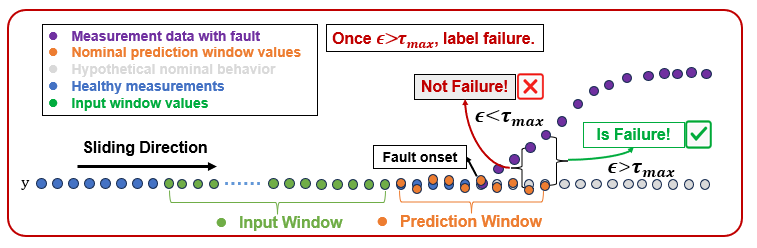
\includegraphics[width=.9\linewidth]{figs/fault_detection.png}
	\caption{Principles of residual-based fault detection}
	\label{fig:fault_detection}
\end{figure}

\rev{In the implemented study, the threshold $\tau_{\mathrm{res}}$ is treated as a hyper-parameter through tuning in a validation set from the source domain. To support the hyper-parameter tuning, we need a few labeled data that are injected through simulation in the source domain. The hyper-parameter tuning is done through optimizing the F1-score:}
\begin{equation}
	{\color{revisionred}
		\tau_{\mathrm{res}}^{\ast}
		=\arg\max_{\tau_{\mathrm{res}}\in\mathcal{T}}
		\mathrm{F1\text{-}score}(\tau_{\mathrm{res}}),}
	\label{eq:threshold_optimization}
\end{equation}
\begin{revision}
	where $\mathcal{T}$ denotes a candidate threshold set. Once determined, $\tau_{\mathrm{res}}^{\ast}$ is fixed and reused in the target domain without target-domain fault labels or re-optimization. Consequently, model training and domain adaptation through transfer learning require healthy data only. We only need a few injected faults in the source domain to support the threshold tuning. Although it is not completely label-free, it can greatly reduce the required labeled data. Especially, we do not require labeled data from the target domain.
	
	In theory, a normal-data-only alternative can also be tested: one could set the threshold as an upper quantile or a statistical confidence bound of the healthy residuals. However, if we do not use labeled fault signals at all, we can only ensure the precision of the detector, but cannot control the recall as we have no information at all on the failed samples. How to achieve balanced detection performance without labeled data remains a challenging issue that deserves future research.
\end{revision}

\rev{It should be noted that the developed fault detection framework relies on the digital twins to create input features. However, a good prediction model does not necessarily guarantee reliable fault detection. In particular, a reliable and robust fault detection model faces the following challenges:}
\begin{enumerate}
	\item \rev{the prediction of the digital twins should be robust against the contamination in the historical observations brought by failure signals and create robust reconstructed residuals. We address this issue through the developed PROF algorithm in Sect. \ref{sec:4.2}};
	\item \rev{the reconstructed residual errors should remain robust against potential shifts from varying operation conditions. In the developed framework, we address this challenge through transfer learning, which is presented in detail in Sect. \ref{sec:4.3}.}
\end{enumerate}
\rev{Overall, the developed fault detection model combines the nominal predictor from the data-driven digital twin, a validation-calibrated residual rule, transfer-based nominal adaptation, and PROF. Their individual contributions are evaluated through ablation studies in Section~\ref{sec:6.2}.}

\subsection{The PROF algorithm}\label{sec:4.2}


Under rolling-horizon operation, the digital twin repeatedly forms new input sliding windows as time advances. As shown in Fig.~\ref{fig:PROF} (a), if a fault-affected measurement is reused as an input, the nominal reconstruction can progressively follow the abnormal trajectory, reducing subsequent residuals and increasing missed detections. To avoid this contamination effect, we develop a new algorithm called fault detection with prediction-based recursive observation feedback (the PROF). The key idea of the PROF algorithm is explained in Fig. \ref{fig:PROF} (b). \rev{PROF addresses the contamination problem while preserving data authenticity by maintaining two separate sequences: the immutable raw monitoring record $\{y_t^{\mathrm{raw}}\}$ used for residual calculation and fault decisions, and an internal buffer recording the data used in the sliding windows for performance prediction $\{\tilde y_t\}$. After the raw observation has been evaluated, the internal buffer is updated as}
\begin{equation}
	{\color{revisionred}\tilde y_t =
		\begin{cases}
			\hat{y}_t,          & \epsilon(t) > \tau_{\mathrm{res}},    \\[6pt]
			y_t^{\mathrm{raw}}, & \epsilon(t) \leq \tau_{\mathrm{res}}.
		\end{cases}}
	\label{eq:prof_update_rule}
\end{equation}

\rev{Due to the sliding-window construction introduced in Section~\ref{sec:3.2}, the corrected internal value affects only future windows whose historical segments contain time $t$. For a future decision index $t'>t$, the target-variable entries of the effective input window are formed from the feedback buffer:}
\begin{equation}
	{\color{revisionred}\boldsymbol{X}_{t'}^{\mathrm{in}}
	=\big[\ldots,\tilde y_{t'-W_{\mathrm{pred}}},\ldots\big],}
	\label{eq:recursive_window}
\end{equation}
\rev{while the decision at $t'$ remains based on $y_{t'}^{\mathrm{raw}}$. PROF therefore never overwrites the archived signal and cannot remove a persistent fault from the decision stream: each new raw sample is evaluated before any feedback-buffer update.}

Fig.~\ref{fig:PROF} illustrates the motivation and effect of the proposed recursive feedback strategy under rolling-horizon operation. After fault onset, fault-affected measurements may not immediately trigger a failure decision if the resulting point-wise residual remains below the detection threshold. Without recursive feedback, as shown in Fig.~\ref{fig:PROF}(a), once a fault is detected at time $t$, the corresponding faulty measurement is directly rolled into subsequent input windows as the prediction horizon advances. This causes the digital twin to gradually follow the faulty trajectory, leading to error propagation and a reduction in point-wise residuals at later decision instants, which may compromise detection reliability.
With PROF, as shown in Fig. ~\ref{fig:PROF} (b), once a fault is detected, the faulty measurement at time $t$ is replaced by its nominal reconstruction before being incorporated into future input windows. This replacement prevents the contamination of historical inputs, stabilizes the rolling-horizon reconstruction of nominal behavior, and preserves the sensitivity of residual-based fault detection over time.
For clarity of illustration, Fig.~\ref{fig:PROF} shows the rolling-horizon operation along the target variable $y$ only, while the actual digital twin operates on multivariate input sequences $\boldsymbol{x}_t$. The gray points indicate hypothetical nominal values that would be observed in the absence of faults and are shown for conceptual reference only; they are not observable in practice and are not used by the proposed method.

\begin{revision}
	The activation boundary of PROF can be stated formally. For a fault beginning at $t_f$, define the first detection time
	\begin{equation}
		t_d=\min\{t\geq t_f:\epsilon(t)>\tau_{\mathrm{res}}\}.
		\label{eq:first_detection_time}
	\end{equation}
	Before $t_d$, abnormal observations are indistinguishable from nominal prediction uncertainty under the current hard decision rule since their signals are too weak and may temporarily enter the feedback buffer. PROF does not retrospectively remove them. From $t_d$ onward, newly detected abnormal values are replaced before the next rolling input is formed, suppressing further recursive contamination. If a weak fault remains below threshold for its entire duration, PROF will not be activated and the fault may be missed. Avoiding this limitation would require a probabilistic or soft-decision extension, with an associated false-alarm trade-off. However, since the fault signals are still weak (otherwise they will be corrected by the PROF), their impacts on the reconstructed reference values will not be very significant. We therefore choose to accept these potential small contamination and design PROF to only correct the more severe faults.
\end{revision}




\begin{figure}
	\centering
	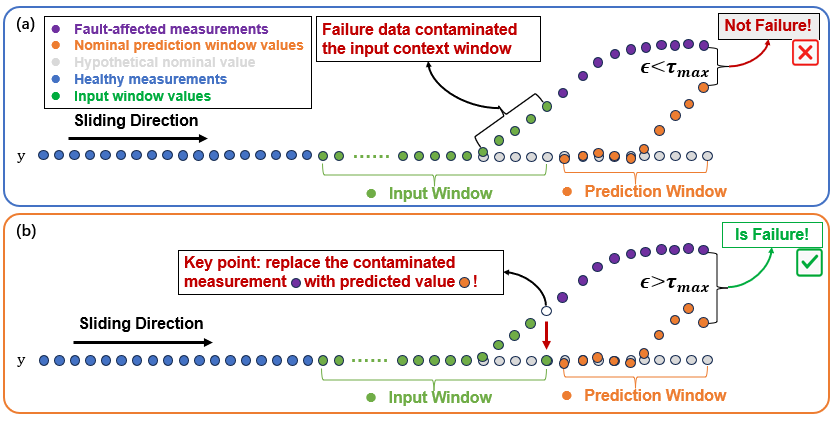
\includegraphics[width=.9\linewidth]{figs/PROF.png}
	\caption{
		Illustration of the PROF mechanism under rolling-horizon operation.
		(a) Without PROF, fault-affected measurements are rolled into subsequent input windows, causing error propagation and suppression of point-wise residuals in later decision steps.
		(b) With PROF, once a fault is detected at time $t$, the fault-affected measurement is replaced by its nominal prediction, preventing error propagation and preserving the sensitivity of residual-based fault detection.
	}
	\label{fig:PROF}
\end{figure}


Overall, PROF integrates (i) point-wise residual-based fault decision at the window end and (ii) recursive observation feedback at the same decision index. This yields a lightweight and robust fault detection mechanism compatible with rolling-horizon digital twin operation, without requiring explicit fault models or labeled fault samples during deployment.



\subsection{Generalization through transfer learning}\label{sec:4.3}

\begin{revision}
	In this paper, we calibrate the decision threshold using source domain validation data, and directly apply it on the target domain. It should be mentioned that this direct reuse can be done only when the monitored quantity, sensing resolution, sampling rate, preprocessing and normalization, residual definition, prediction horizon, and fault decision semantics remain unchanged. In addition, the target nominal model must be adapted with verified healthy data so that its fault-free residual scale is comparable with the source residual scale. In particular, we should be able to demonstrate that after the transfer learning on the predictive digital twin, the distributions of the residual errors between the reconstructed reference values and the actual measurements are close enough so that a threshold calibrated based on the residual distribution on the source domain can be safely applied on the target domain. These conditions hold for the two ArmPi robots used as case study in this paper. Section~\ref{sec:6.1} verifies the domain shift and shows that transfer learning concentrates target residuals around zero; Section~\ref{sec:6.2.1} reports the threshold-sensitivity curve. Threshold reuse is not asserted for sensors, sampling protocols, fault modes, or operating envelopes that violate these conditions.

	An above-threshold residual establishes a model--system inconsistency, but does not by itself identify its physical cause. The proposed operational logic therefore separates detection from diagnosis. A transient or persistent exceedance first triggers an abnormal-state flag and quarantines the associated observations from any model update. Maintenance evidence, additional sensors, or controlled inspection is then required to distinguish (i) a fault or incipient abnormality, for which the model remains fixed and fault-handling action is taken, from (ii) verified healthy evolution or model inadequacy, for which a new healthy batch may be collected and the digital twin updated at low frequency. This conservative logic prevents suspected-fault data from being learned as nominal behavior, while acknowledging that fully automatic fault-versus-drift diagnosis is beyond the present residual detector.

	If the aforementioned prerequisite does not hold, especially, when the residual distributions differ significantly between the source and target domains, transfer learning can be applied again to update the optimal values of the detection threshold.
\end{revision}



\section{Experiment design}\label{sec:5}

The proposed digital twin modeling and fault detection framework is validated on a real robotic platform.
Section~\ref{sec:5.1} introduces the experimental setup and system configuration.
Section~\ref{sec:5.2} describes the digital twin modeling implementation.
Section \ref{sec:5-sensitivity} presents a study demonstrating the strength of the DoE over traditional random sampling.
Section~\ref{sec:5.3} details the fault detection experiments based on the PROF mechanism.


\subsection{Experimental robotic digital twin platform}\label{sec:5.1}

To support the development and experimental validation of the proposed data-driven digital twin framework, an open-source robotic demonstration platform was used.
The platform integrates a ROS-based physical robotic system with a Simulink-based virtual robotic model, enabling real-time condition monitoring, data-driven digital twin modeling, and decision support.
This platform provides the experimental foundation for the modeling, updating, and evaluation methods introduced in the subsequent sections.
An overview of the platform architecture is shown in Fig.~\ref{fig:platform_structure}, and its main components are described below.

\begin{figure}
	\centering
	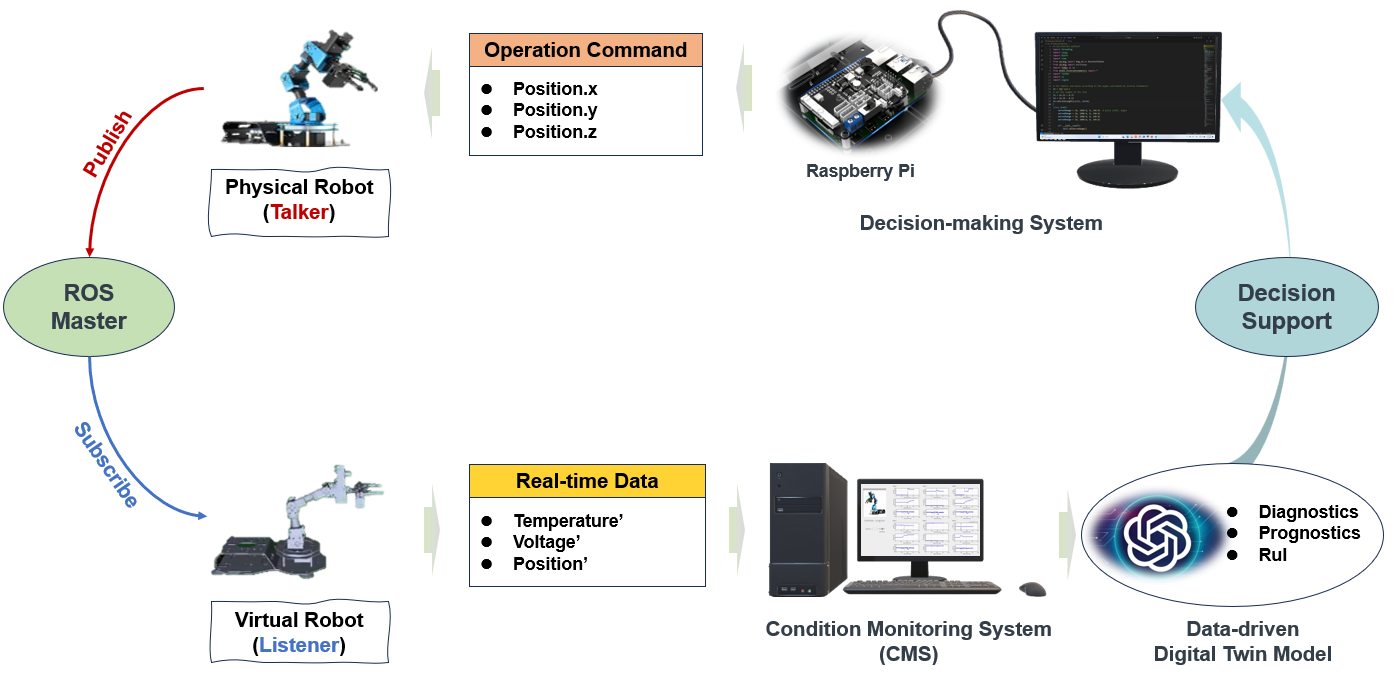
\includegraphics[width=0.9\textwidth]{figs/platform_structure.png}
	\caption{Overview of the robotic digital twin platform and its components.}
	\label{fig:platform_structure}
\end{figure}

\textbf{A six-degree-of-freedom ArmPi robotic arm} serves as the physical experimental platform in this study, as illustrated in Fig.~\ref{fig:robot_structure}.
The robot is compatible with ROS, with each joint driven by a smart serial bus servo motor.
These actuators provide real-time feedback on joint position, temperature, and voltage, resulting in a total of 18 sensor signals.
The robotic arm executes pick-and-place operations and trajectory tracking tasks based on inverse kinematics control.

\begin{figure}
	\centering
	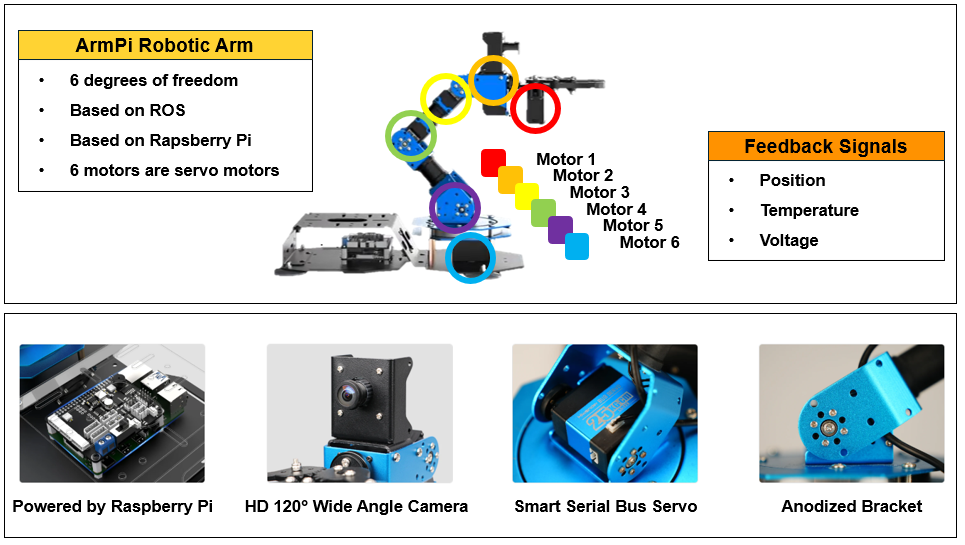
\includegraphics[width=0.8\textwidth]{figs/robot_structure.png}
	\caption{Structure and components of the ArmPi robotic arm.}
	\label{fig:robot_structure}
\end{figure}


\textbf{A condition monitoring system (CMS)}, implemented to acquire and process multisensor data from the physical robot via ROS.
The CMS subscribes to joint position, motor temperature, and motor voltage signals, assigns synchronized timestamps, and supports subsequent digital twin modeling.
The monitored parameters are summarized in Table~\ref{tab:cms_parameters}. All source code and datasets generated using this experimental platform are publicly available at:
\url{https://github.com/sonic160/digital_twin_robot}.

\begin{table*}[htbp]
	\centering
	\caption{Condition monitoring parameters.}
	\label{tab:cms_parameters}
	\begin{tabular}{p{0.15\textwidth}p{0.15\textwidth}p{0.1\textwidth}p{0.5\textwidth}}
		\toprule
		\textbf{Parameter Name} & \textbf{Symbol} & \textbf{Unit}       & \textbf{Description}                \\
		\midrule
		Temperature             & $T$             & $\mathrm{^\circ C}$ & Motor temperature during operation. \\
		Voltage                 & $V$             & V                   & Motor working voltage.              \\
		Position                & $P$             & /                   & Joint position of the motor.        \\
		\bottomrule
	\end{tabular}
\end{table*}



%
% Experimental setup and design
%
\subsection{Data-driven digital twin modeling}\label{sec:5.2}

In this study, to validate the data-driven digital twin modeling and updating framework introduced in the previous sections, two robots in Fig.~\ref{fig:robot_structure} with different levels of motor degradation, were configured as experimental platforms. We train a data-driven digital twin on one robot (referred to as source robot), and test the model updating through transfer learning on the other robot (referred to as target robot). This configuration serves as a controlled experimental setting for validating the proposed digital twin construction, rolling horizon prediction, and transfer learning based updating strategy. The corresponding task structure, sampling strategy, and data collection process that implement the experiment design discussed earlier are illustrated in Fig.~\ref{fig:experiment_design}.

To enable the collection of diverse and representative data for model development, a set of pick and place tasks was systematically designed to generate representative operational data. As illustrated in Fig.~\ref{fig:experiment_design}, each task consists of five sequential movements: returning to the initial position, moving to the pick up location, grasping the object, transporting it to the placement location, and releasing the object. For each task, the pick up and placement positions are predefined, and the corresponding joint trajectories are computed through inverse kinematics to ensure physical feasibility. During execution, sensor data including motor position, voltage, and temperature are collected at a frequency of 10~Hz, providing time series measurements of system behavior under various task conditions.

\begin{figure}
	\centering
	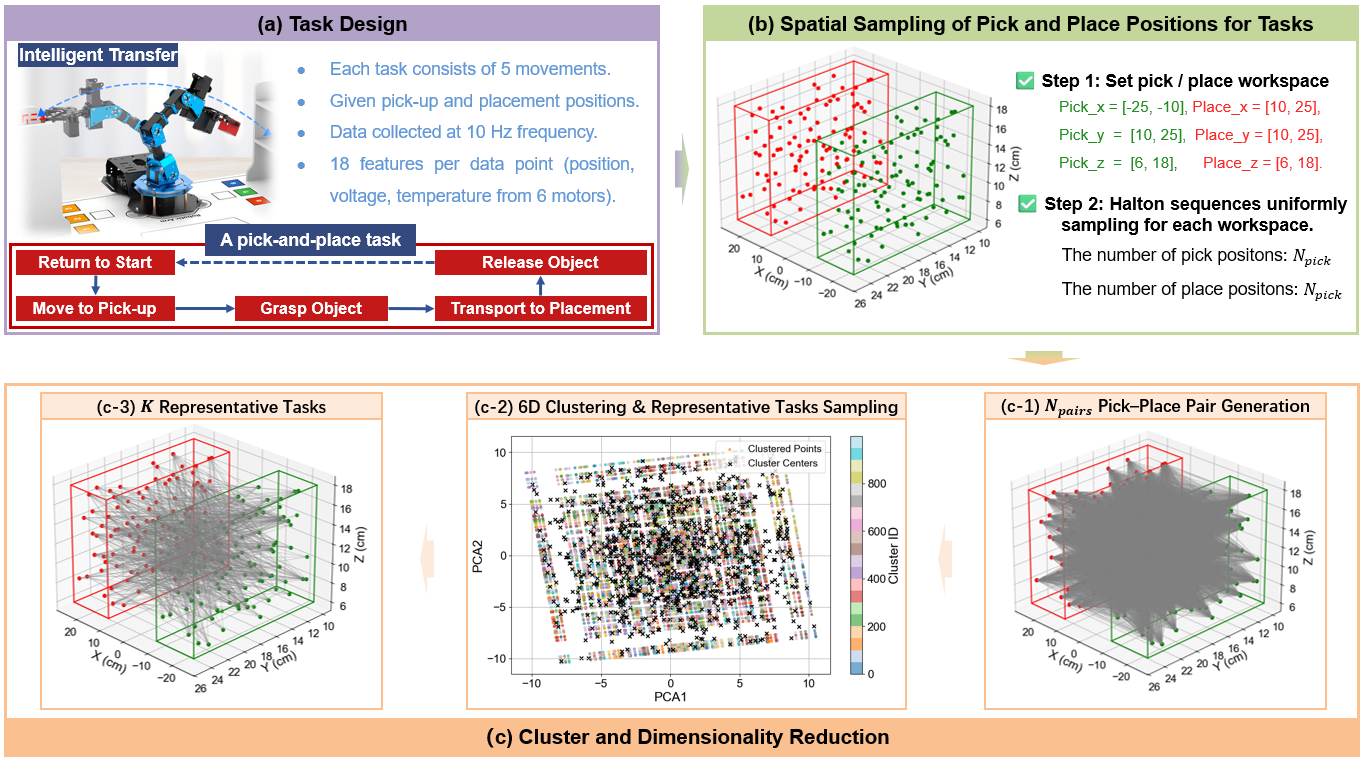
\includegraphics[width=1\linewidth]{figs/experiment_design.png}
	\caption{Task Design and Sampling Strategy for Robotic Pick and Place Experiments}
	\label{fig:experiment_design}
\end{figure}

\rev{The sampled space is the predefined feasible Cartesian pick-and-place envelope, rather than the complete dynamic state space of the robot. As shown in Fig.~\ref{fig:experiment_design}(b), its spatial boundaries were defined from workspace and safety constraints. A Halton low-discrepancy design generated $N_{\text{pick}}=100$ pick points and $N_{\text{place}}=100$ place points. Executing the resulting feasible trajectories then produced diverse joint-level temporal responses. The design is intended to improve representative task-space coverage under a fixed sampling budget; it does not guarantee exhaustive coverage of every operating condition.}

By connecting all possible combinations of the 100 pick positions and 100 place positions, a total of \(100 \times 100 = 10{,}000\) candidate pick place task pairs were generated. Each pair was validated through inverse kinematics to ensure feasibility, resulting in \(N_{\text{pairs}}=10{,}000\) valid task trajectories. As illustrated in Fig.~\ref{fig:experiment_design}(c), a clustering based sampling strategy was then applied to reduce redundancy and enhance diversity. Each task pair was encoded as a six-dimensional vector based on the spatial coordinates of the pick and place positions. MiniBatch K Means clustering was performed to partition the 10,000 task samples into \(K=1,270\) clusters. To facilitate visualization and diversity assessment, the high dimensional vectors were projected into a 2D space using principal component analysis (PCA). From each cluster, a representative task was selected by identifying the sample closest to the cluster center, resulting in a final set of 1,270 representative pick place trajectories that uniformly span the task space and are used for subsequent data collection and model training.

The source and target robots executed the selected representative pick and place tasks, generating the corresponding source domain dataset \( D_{\text{src}} \) and target domain dataset \( D_{\text{tgt}} \), respectively. A total of $K_{\text{src}}=1000$ tasks and $K_{\text{tgt}}=270$ tasks were performed by the source and target robots, ensuring diversity while maintaining task consistency across platforms. During task execution, the condition monitoring system (CMS) collected 18 dimensional multivariate time series data including position, temperature, and voltage signals from six motors at a sampling rate of 10 Hz. This resulted in a total of 10,400 seconds (i.e., 104,000 data points) of data for the source robot and 1,404 seconds (i.e., 14,040 data points) for the target robot, yielding two platform specific datasets: $D_{\mathrm{src}}\in\mathbb{R}^{104000\times18}$ and $D_{\mathrm{tgt}}\in\mathbb{R}^{14040\times18}$. To support model development and evaluation, the datasets were partitioned into training, validation, and testing subsets without shuffling to preserve temporal dependencies. Specifically, $D_{\mathrm{src}}$ was split into $\mathcal{D}_{\mathrm{src}}^{\mathrm{train}}$, $\mathcal{D}_{\mathrm{src}}^{\mathrm{val}}$, and $\mathcal{D}_{\mathrm{src}}^{\mathrm{test}}$ using a ratio of 7:1.5:1.5. Similarly, $D_{\mathrm{tgt}}$ was divided into $\mathcal{D}_{\mathrm{tgt}}^{\mathrm{train}}$ and $\mathcal{D}_{\mathrm{tgt}}^{\mathrm{test}}$ with a ratio of 8:1, as summarized in Table~\ref{tab:dataset_sample_fault_summary}.

\begin{table}[pos=htbp]
	\centering
	\caption{Summary of dataset partitions and fault injection statistics}
	\label{tab:dataset_sample_fault_summary}
	\renewcommand{\arraystretch}{1.2}
	\begin{tabular}{lllllp{5.2cm}<{\raggedright\arraybackslash}}
		\toprule
		\textbf{Dataset Name}                              & \textbf{Domain} & \textbf{Type}  & \textbf{Total Points} & \textbf{Total Samples} & \textbf{Description}                                  \\
		\midrule
		\( \mathcal{D}_{\text{src}}^{\text{train}} \)      & Source          & Normal         & 72,800                & 72,761                 & Source domain training set (normal data)              \\
		\( \mathcal{D}_{\text{src}}^{\text{val}} \)        & Source          & Normal         & 15,600                & 15,561                 & Source domain validation set (normal data)            \\
		\( \mathcal{D}_{\text{src}}^{\text{test}} \)       & Source          & Normal         & 15,600                & 15,561                 & Source domain test set (normal data)                  \\
		\( \mathcal{D}_{\text{tgt}}^{\text{train}} \)      & Target          & Normal         & 12,480                & 12,441                 & Target domain training set (normal data)              \\
		\( \mathcal{D}_{\text{tgt}}^{\text{test}} \)       & Target          & Normal         & 1,560                 & 1,521                  & Target domain test set (normal data)                  \\
		\midrule
		\( \mathcal{D}_{\text{src}}^{\text{val-fault}} \)  & Source          & Fault-injected & 15,600                & 15,561                 & Source domain validation set with fault-injected data \\
		\( \mathcal{D}_{\text{src}}^{\text{test-fault}} \) & Source          & Fault-injected & 15,600                & 15,561                 & Source domain test set with fault-injected data       \\
		\( \mathcal{D}_{\text{tgt}}^{\text{test-fault}} \) & Target          & Fault-injected & 1,560                 & 1,521                  & Target domain test set with fault-injected data       \\
		\bottomrule
	\end{tabular}
\end{table}

\subsection{Task-space coverage and domain-shift characterization}\label{sec:5-sensitivity}

\begin{revision}
	The performance of the DoE through Halton sequences is evaluated at the stage where it acts directly: we evaluate the coverage of normalized Cartesian task coordinates under a given sample budget. We use centered discrepancy $D_c$ (smaller is better) to measure multidimensional deviation from a uniform coverage and average two-dimensional projected grid coverage $C_{2\mathrm{D}}$ (larger is better) to measure how broadly pairwise projections occupy the feasible region. We choose random sampling as a baseline as it is widely-used to generate training data in the current data-driven digital twin studies. Random sampling is repeated with three independent seeds; the deterministic Halton design is reported once. Table~\ref{tab:doe_coverage} shows substantially lower discrepancy and higher projected coverage for both pick and place regions. This supports the proposed methods as a space-filling task design.
\end{revision}

\begin{table}[pos=htbp]
	\centering
	\color{revisionred}
	\caption{\color{revisionred}Task-space coverage under an identical sampling budget. Random results are mean $\pm$ SD over three seeds.}
	\label{tab:doe_coverage}
	\begin{tabular}{llcc}
		\toprule
		Method & Region & Centered discrepancy $\downarrow$ & Avg. 2D coverage $\uparrow$ \\
		\midrule
		Random & Pick   & $0.005294\pm0.003099$             & $0.6322\pm0.0259$           \\
		Random & Place  & $0.007692\pm0.003922$             & $0.6256\pm0.0195$           \\
		Halton & Pick   & $0.000271$                        & $0.7567$                    \\
		Halton & Place  & $0.000271$                        & $0.7567$                    \\
		\bottomrule
	\end{tabular}
\end{table}

\begin{revision}
	To quantify the source-to-target shift, Table~\ref{tab:domain_shift} compares motor~6 measurements. Temperature and voltage exhibit large standardized mean differences and Kolmogorov--Smirnov (KS) statistics, whereas motor position remains closely matched. The two robots therefore execute comparable motion configurations but differ markedly in electrical and thermal responses, which motivates nominal-model adaptation rather than attributing the target degradation solely to a different task distribution.
\end{revision}

\begin{table}[pos=htbp]
	\centering
	\color{revisionred}
	\caption{\color{revisionred}Statistical comparison of motor~6 variables between source and target domains.}
	\label{tab:domain_shift}
	\begin{tabular}{lccc}
		\toprule
		Indicator               & Temperature ($^\circ$C) & Voltage           & Position          \\
		\midrule
		Source mean $\pm$ SD    & $40.13\pm1.48$          & $7246.56\pm47.90$ & $644.54\pm172.33$ \\
		Target mean $\pm$ SD    & $43.25\pm1.84$          & $7404.93\pm38.67$ & $642.21\pm167.52$ \\
		Mean difference         & $+3.12$                 & $+158.38$         & $-2.33$           \\
		KS statistic            & $0.671$                 & $0.937$           & $0.029$           \\
		Standardized difference & $1.87$                  & $3.64$            & $-0.014$          \\
		\bottomrule
	\end{tabular}
\end{table}

\rev{The LSTM defined in Section~\ref{sec:3.2.3} learns a data-driven digital twin from the source-domain training data $\mathcal{D}_{\text{src}}^{\text{train}}$ and is subsequently evaluated and adapted in the target domain. Consistent with the sample construction above, the predictor estimates motor~6 temperature from the 18 measured covariates. The developed methods and baselines are compared using $R^2$, MAPE, RMSE, and MSE in Section~\ref{sec:6.1}.}

Figure~\ref{fig:domain_distribution} illustrates the joint distribution of motor~6 position, voltage, and temperature in the source and target domains. Compared to the source domain, the target domain exhibits a higher concentration of temperature values in the upper range and a distinct shift in voltage position correlation. Such discrepancies may contribute to the degradation of model generalization when transferred across domains, and they provide an empirical basis for evaluating the digital twin updating strategy in the subsequent analysis.

%
% Fault detection through the PROF algorithm
%
\subsection{Fault injection and detection through the PROF algorithm}\label{sec:5.3}

\rev{In this work, we inject faults related to abnormal temperature rise through simulation to test the developed fault detection methods. Simulation is chosen instead of physical fault injection mainly because injecting real faults risks damaging the robots and raises safety and budget concerns. To model the temperature response of an electric motor under an abnormal temperature rise such as that caused by rotor stall, we adopt a first-order lumped-parameter thermal network (LPTN) \citep{khalesidoost2022overview, sciascera2017analytical, boglietti2009evolution, ramarathnam2015review}.} Based on this model, transient thermal faults were synthetically injected into the temperature signals of motor 6 using a semi-empirical formulation to simulate realistic degradation scenarios (see Eq.~\eqref{eq:combined}). The thermal dynamics are governed by:

\begin{equation}
	C_{\mathrm{th}} \cdot \frac{dT(t)}{dt} + \frac{T(t) - T_{\mathrm{env}}}{R_{\mathrm{th}}} = P(t)
	\label{eq:lptn_base}
\end{equation}
where \( T(t) \) is the system temperature, \( T_{\mathrm{env}} \) is the ambient temperature, \( C_{\mathrm{th}} \) is the thermal capacitance, \( R_{\mathrm{th}} \) is the thermal resistance, and \( P(t) \) is the thermal power input. The thermal time constant is defined as:

\[
	\tau = R_{\mathrm{th}} \cdot C_{\mathrm{th}}
\]

Assuming a constant power input \( P(t) = P_{\mathrm{fault}} \) during the fault period, Equation~\eqref{eq:lptn_base} has the analytical solution:

\begin{equation}
	T(t) = T_{\infty} - \left( T_{\infty} - T_0 \right) e^{-t/\tau}, \quad \text{where} \quad T_{\infty} = T_{\mathrm{env}} + R_{\mathrm{th}} \cdot P_{\mathrm{fault}}
	\label{eq:heating}
\end{equation}
Here, \( T_0 \) is the initial temperature, and \( T_{\infty} \) is the theoretical steady state temperature.

After fault removal at time \( t = t_{\mathrm{cool}} \), the power input drops to zero, i.e., \( P(t) = 0 \). The system then enters a natural cooling process governed by:

\begin{equation}
	T(t) = T_{\mathrm{env}} + \left( T_{\mathrm{peak}} - T_{\mathrm{env}} \right) e^{-(t - t_{\mathrm{cool}})/\tau}
	\label{eq:cooling}
\end{equation}
where \( T_{\mathrm{peak}} = T(t_{\mathrm{cool}}) \) is the temperature at the moment the fault is repaired. The full temperature profile \( T(t) \), including both heating and cooling stages, can be expressed as a piecewise function:

\begin{equation}
	T(t) =
	\begin{cases}
		T_{\infty} - (T_{\infty} - T_0) e^{-t/\tau},                                                 & t < t_{\mathrm{cool}}    \\[6pt]
		T_{\mathrm{env}} + (T_{\mathrm{peak}} - T_{\mathrm{env}}) e^{-(t - t_{\mathrm{cool}})/\tau}, & t \geq t_{\mathrm{cool}}
	\end{cases}
	\label{eq:combined}
\end{equation}

\begin{revision}
	The injected failure signals represent a physically-motivated progressive thermal anomaly rather than a complete electromechanical simulation of a specific failure. An additional heat input produces first-order heating and its removal produces exponential cooling, consistent with the dominant temperature consequence of temporary overload, increased mechanical friction, restricted cooling, or short-duration jamming. The construction is preferred to an arbitrary step or random perturbation because onset, amplitude, duration, and recovery remain interpretable and repeatable.

	\rev{Faults spanning 30--50 samples and reaching 4--8\,$^\circ$C above the nominal trajectory were inserted into the source validation and test sets and the target test set. With the 1\,$^\circ$C sensor resolution, a point was labeled faulty only when the injected trajectory exceeded its baseline by more than 1\,$^\circ$C. The saved evaluation files contain 676 labeled decision points in each source fault subset and 164 in $\mathcal{D}_{\mathrm{tgt}}^{\mathrm{test-fault}}$ after rolling-window alignment. The training of the data-driven digital twins and its adaptation to the target domain used only fault-free data. The threshold was calibrated only on $\mathcal{D}_{\mathrm{src}}^{\mathrm{val-fault}}$ and then fixed.}

	It should be noted that real motor failures can additionally involve time-varying load, speed, ambient conditions, nonlinear heat transfer, controller intervention, and electrical, mechanical, or vibration signatures that are not represented by the first-order LPTN. The present experiment therefore validates detection of transient or gradually developing overheating anomalies, not every motor failure mode or root-cause diagnosis. Non-thermal, highly intermittent, or temperature-unobservable faults lie outside the current validation boundary; naturally occurring or safely reproduced physical faults remain future work. However, the developed framework remains applicable to real motor failures, as long as we can collect training data from real experiments. In this case, we just need to replace the injected failure with the actual failure data.
\end{revision}

\begin{figure}
	\centering
	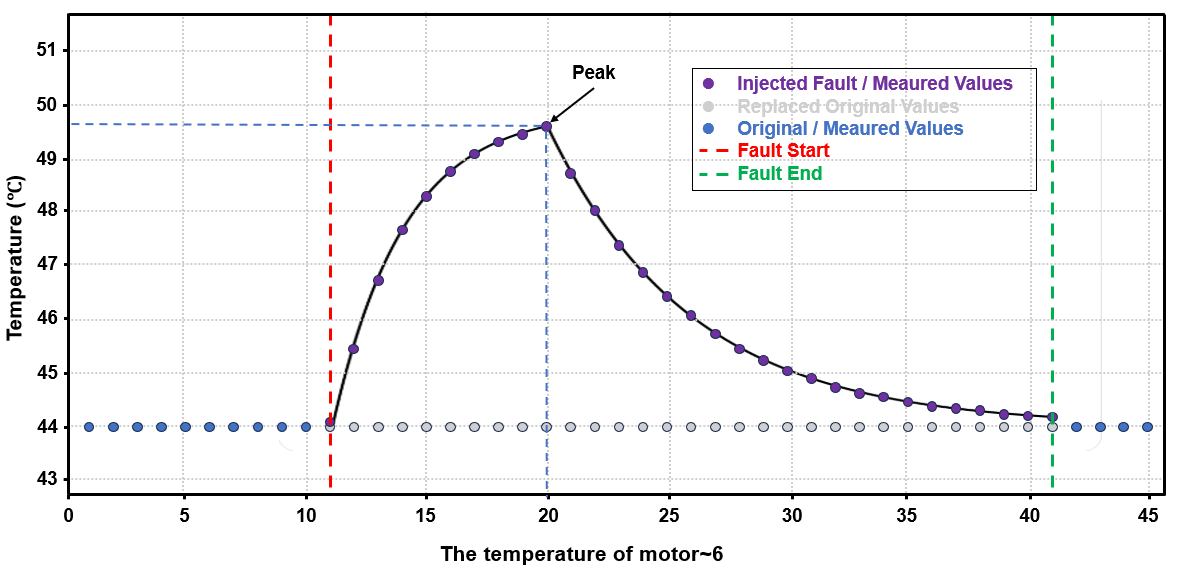
\includegraphics[width=0.9\linewidth]{figs/semi-empirical.png}
	\caption{Synthetic motor temperature trajectory based on LPTN}
	\label{fig:semi-empiricall}
\end{figure}



\begin{figure}
	\centering
	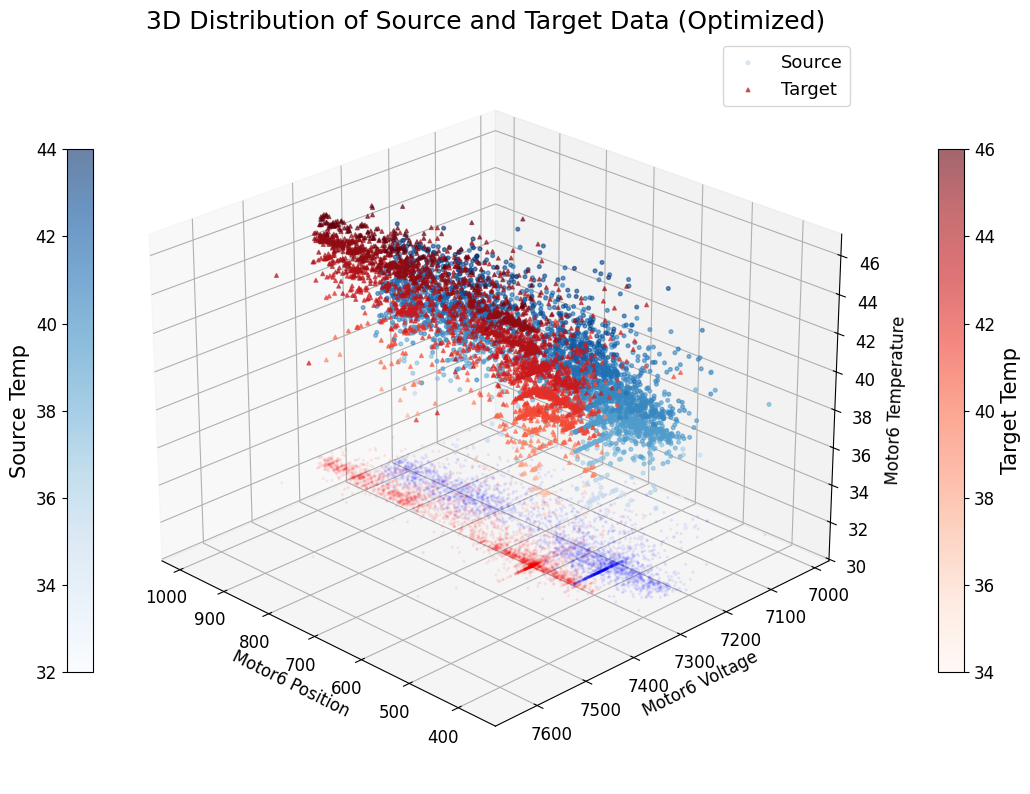
\includegraphics[width=0.8\linewidth]{figs/domain_distribution.png}
	\caption{Cross Domain Distribution of Motor~6 Signals}
	\label{fig:domain_distribution}
\end{figure}


\section{Results and discussions}\label{sec:6}

This section presents a comprehensive evaluation of the proposed framework.
Section~\ref{sec:6.1} first analyzes the performance of data-driven digital twin modeling in both source and target domains.
Section~\ref{sec:6.2} then investigates residual-based fault detection performance, including threshold calibration, transfer learning effects, and the factorial ablation of PROF and transfer learning. \rev{Section~\ref{sec:6.3} reports inference latency and target-domain fine-tuning time.}




\subsection{Data-driven digital twin modeling performance}
\label{sec:6.1}

The objective of this section is to assess how accurately the data-driven digital twin can model the nominal thermal behavior of motor~6, and if the developed transfer learning strategy can update the digital twin model to adapt to changes.


Following the data-driven digital twin modeling procedure described in Section~\ref{sec:3},
the multivariate observation of the system at discrete time $t$ is denoted by the vector $\boldsymbol{x}_t$.
The target variable $y_t$ is extracted from the multivariate observation via a projection operator $\pi(\cdot)$, i.e., $y_t = \pi(\boldsymbol{x}_t)$.
In the experimental setting considered in this work, the observation vector $\boldsymbol{x}_t$ is constructed by combining temperature, joint position, and working voltage measurements collected from six motors, resulting in an 18-dimensional multivariate representation.
In this work, the target variable $y_t$ corresponds to the temperature of motor~6.


Supervised learning samples are constructed using a sliding-window strategy.
For each sample aligned with the current time index $t$, the input context window
$\boldsymbol{X}_t^{\mathrm{in}}$ consists of an ordered sequence of historical
observations preceding the prediction interval.
Under the experimental parameter setting adopted in this study, the input
window contains $30$ consecutive time steps and the prediction lead time is 10. Therefore, we have
$
	\boldsymbol{X}_t^{\mathrm{in}}
	=
	\big[
		\boldsymbol{x}_{t-39},\ldots,\boldsymbol{x}_{t-10}
		\big]^\top .$



The corresponding output window $\boldsymbol{y}_t^{\mathrm{pred}}$ represents the
nominal trajectory of the target variable aligned with time $t$, corresponding
to the digital twin's nominal estimation over the most recent $10$ time steps:
$\boldsymbol{y}_t^{\mathrm{pred}}
	=
	\big[
		\hat{y}_{t-9},\ldots,\hat{y}_t
		\big]^\top .$
Since the target variable $y_t$ is instantiated
as the temperature of motor~6, the above definition can be equivalently written as the $10$-step nominal temperature reconstruction
$\boldsymbol{y}_t^{\mathrm{pred}}
	=
	\big[
		\hat{T}_6(t-9),\ldots,\hat{T}_6(t)
		\big]^\top .$
As each sample spans 40 consecutive time steps, the total number of available samples is reduced by 39 relative to the number of raw time points in the dataset. The resulting sample counts for all datasets are summarized in Table~\ref{tab:dataset_sample_fault_summary}.

A three-layer Long Short-Term Memory (LSTM) network is used to model the nonlinear temporal relationships in the multivariate system dynamics. The network architecture and training hyperparameters are summarized in Table~\ref{tab:model_parameters}. In all experiments, early stopping based on validation loss is employed to prevent overfitting.

\begin{table*}[htbp]
	\caption{Model hyperparameters and descriptions}
	\centering
	\label{tab:model_parameters}
	\begin{tabular}{@{}p{0.25\textwidth}p{0.15\textwidth}p{0.5\textwidth}@{}}
		\toprule
		\textbf{Parameter Name} & \textbf{Value} & \textbf{Description}                                     \\
		\midrule
		Input\_dim / \(d\)      & (30, 18)       & The number of input features for each time step in LSTM. \\
		Hidden\_dim / \(h\)     & 256            & The number of hidden units in the LSTM layer.            \\
		Output\_dim             & (10, 1)        & The number of future time steps to predict.              \\
		Num\_layers             & 3              & The number of stacked LSTM layers in the model.          \\
		Dropout                 & 0.2            & Dropout rate between LSTM layers to prevent overfitting. \\
		Epochs                  & 100            & The maximum number of training epochs.                   \\
		Learning\_rate          & 0.0001         & Learning rate for Adam optimizer.                        \\
		Loss\_function          & MSELoss        & Loss between predictions and ground truth.               \\
		Optimizer               & Adam           & Optimizer used to update model parameters.               \\
		\bottomrule
	\end{tabular}
\end{table*}



\subsubsection{Source-domain nominal modeling}

We first evaluate the digital twin modeling performance in the source domain. The LSTM-based digital twin is trained using the source-domain training dataset \( \mathcal{D}_{\text{src}}^{\text{train}} \), validated on \( \mathcal{D}_{\text{src}}^{\text{val}} \), and finally evaluated on the held-out test dataset \( \mathcal{D}_{\text{src}}^{\text{test}} \).

\begin{revision}
	Before subsequent transfer-learning and fault-detection experiments, the selection of the forecasting backbone was examined under a controlled protocol. The LSTM is compared with two other commonly-used machine learning regression models, \emph{i.e.,} Transformer and XGBoost. All the three models were trained using all 104,000 source-domain observations, the same chronological 70\%/15\%/15\% split, the same 18 variables, a 30-step history, a direct 10-step output, and the same held-out test set. Neural models used batch size 64, at most 100 epochs, patience 10, dropout 0.2, Adam, and MSE loss. XGBoost received the identical $30\times18$ history flattened to 540 features and predicted the same ten outputs; only algorithm-specific optimization settings differed.
\end{revision}

\begin{table}[pos=H]
	\centering
	\color{revisionred}
	\caption{\color{revisionred}Controlled source-domain nominal-model comparison on the held-out test set (seed 42).}
	\label{tab:source_model_comparison}
	\begin{tabular}{lccccc}
		\toprule
		Model       & RMSE            & $R^2$           & MAPE (\%)       & Train (s)     & Size (MB)     \\
		\midrule
		LSTM        & 0.4411          & 0.8591          & 0.7550          & 147.5         & \textbf{0.36} \\
		XGBoost     & \textbf{0.4239} & \textbf{0.8699} & \textbf{0.7235} & \textbf{36.7} & 24.38         \\
		Transformer & 0.4430          & 0.8579          & 0.7651          & 598.8         & 0.43          \\
		\bottomrule
	\end{tabular}
\end{table}

\begin{figure}[pos=H]
	\centering
	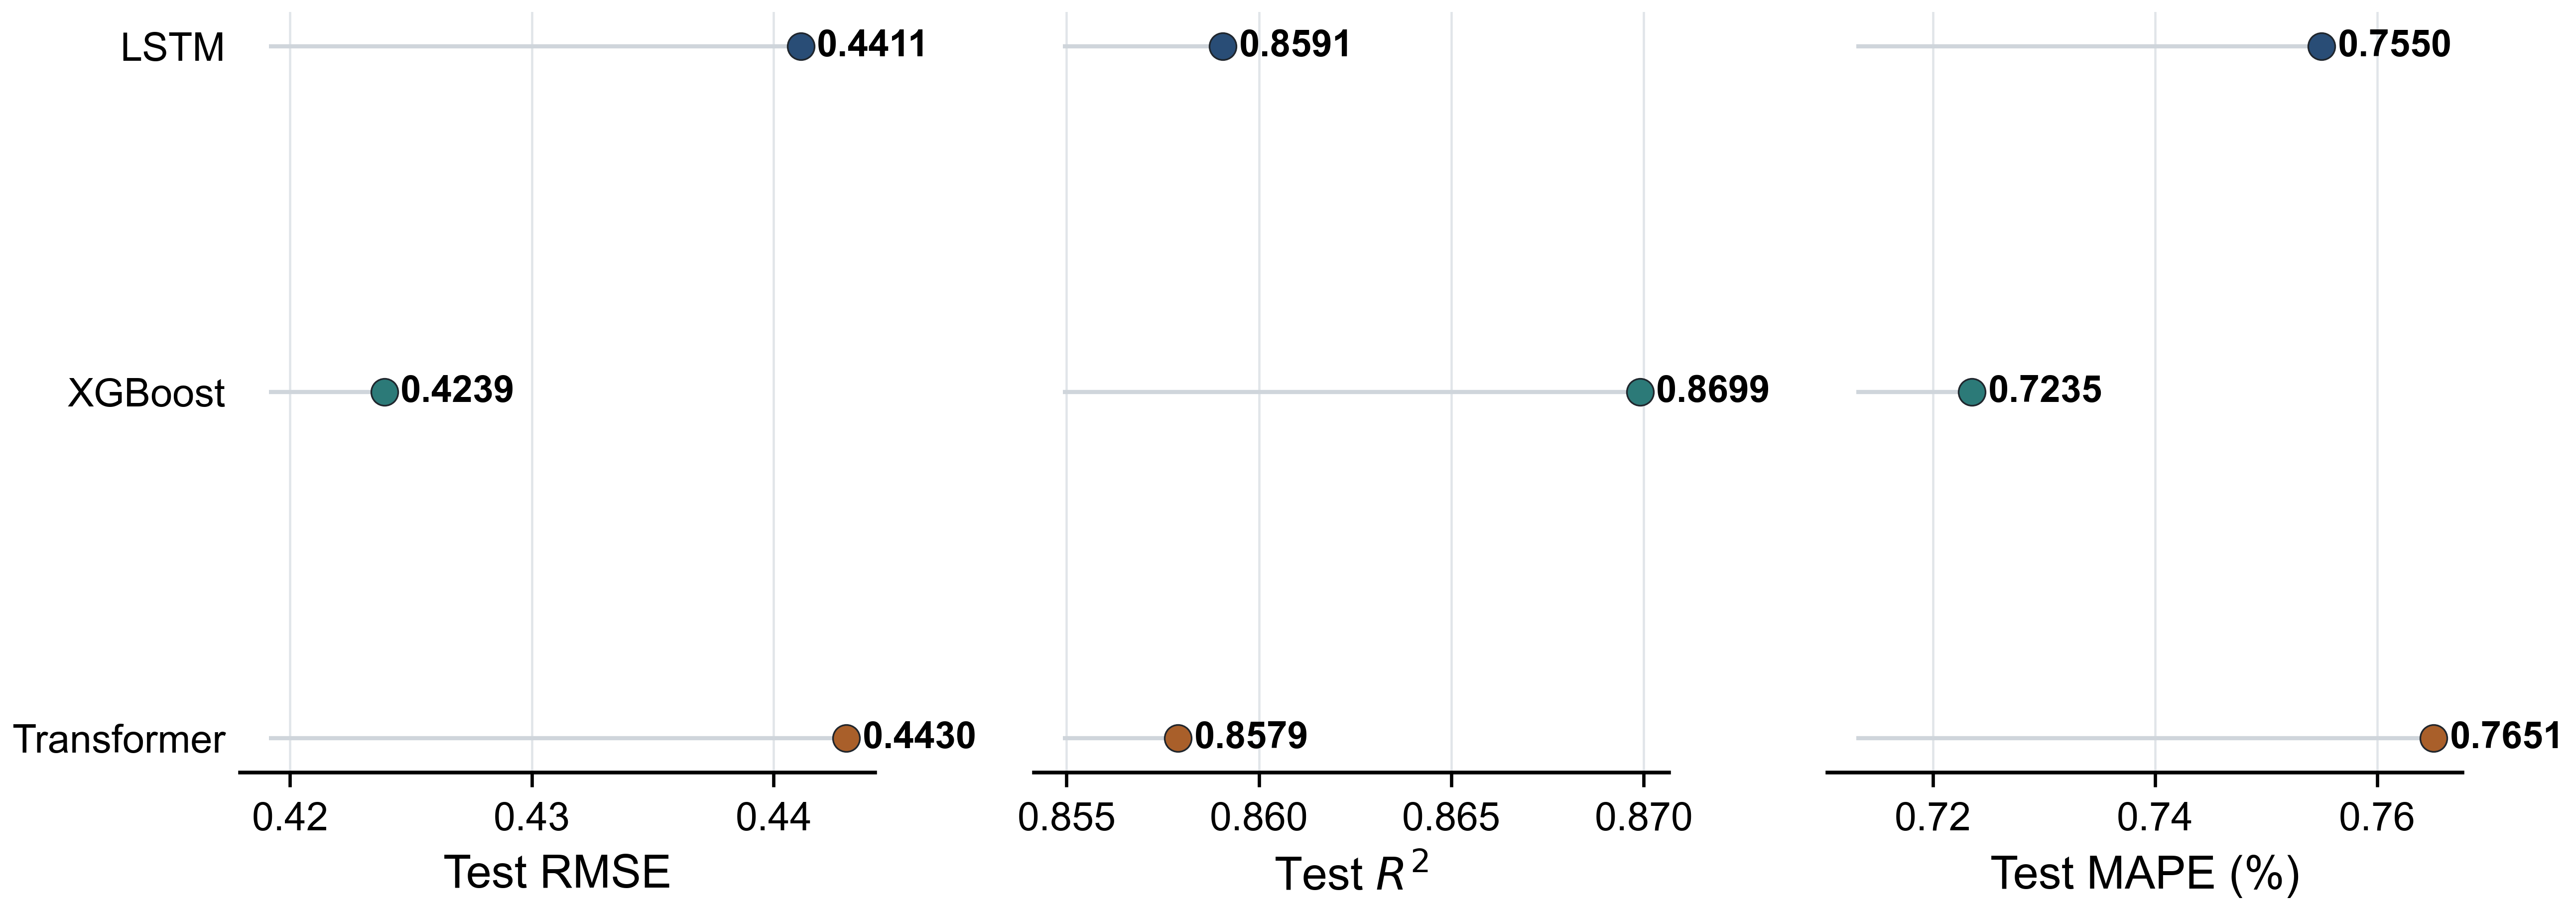
\includegraphics[width=.96\linewidth]{figs/source_model_accuracy_publication.png}
	\caption{\rev{Source-domain nominal-model accuracy comparisons.}}
	\label{fig:source_model_comparison}
\end{figure}

\begin{revision}
	Table~\ref{tab:source_model_comparison} and Fig.~\ref{fig:source_model_comparison} show that XGBoost gives the best point estimate, with an $R^2$ advantage of 0.0108 over the archived LSTM checkpoint, but its model is substantially larger. LSTM requires 147.5~s to train, longer than XGBoost (36.7~s) but substantially shorter than Transformer (598.8~s). Transformer has a similar point estimate to LSTM. LSTM is retained because it combines competitive accuracy with the smallest footprint, the lowest batch-1 inference latency reported in Section~\ref{sec:6.3}, a moderate offline training cost, and direct compatibility with the layer-wise parameter-transfer procedure. The archived LSTM checkpoint is used consistently throughout the source prediction, direct-generalization, and transfer-learning analyses; XGBoost and Transformer are not carried into downstream adaptation. The framework itself is independent of the forecasting architecture and can use another temporal predictor, provided that it supports rolling prediction and generates the nominal reference required for residual calculation and PROF.

	We also tested history lengths $W_{\mathrm{in}}\in\{20,30,40,50,60\}$ with prediction horizons $W_{\mathrm{pred}}\in\{10,15,20,25,30\}$. Figure~\ref{fig:window_sensitivity} shows that a longer history does not monotonically improve either $R^2$ or MSE. At the retained horizon $W_{\mathrm{pred}}=10$, prediction performance is stable across the tested history lengths and the 30-step setting is near-optimal. We therefore use the fixed setting $W_{\mathrm{in}}=30$ and $W_{\mathrm{pred}}=10$ for all models, preserving a consistent temporal structure without introducing the additional complexity of adaptive window selection.
\end{revision}

\begin{figure}[pos=H]
	\centering
	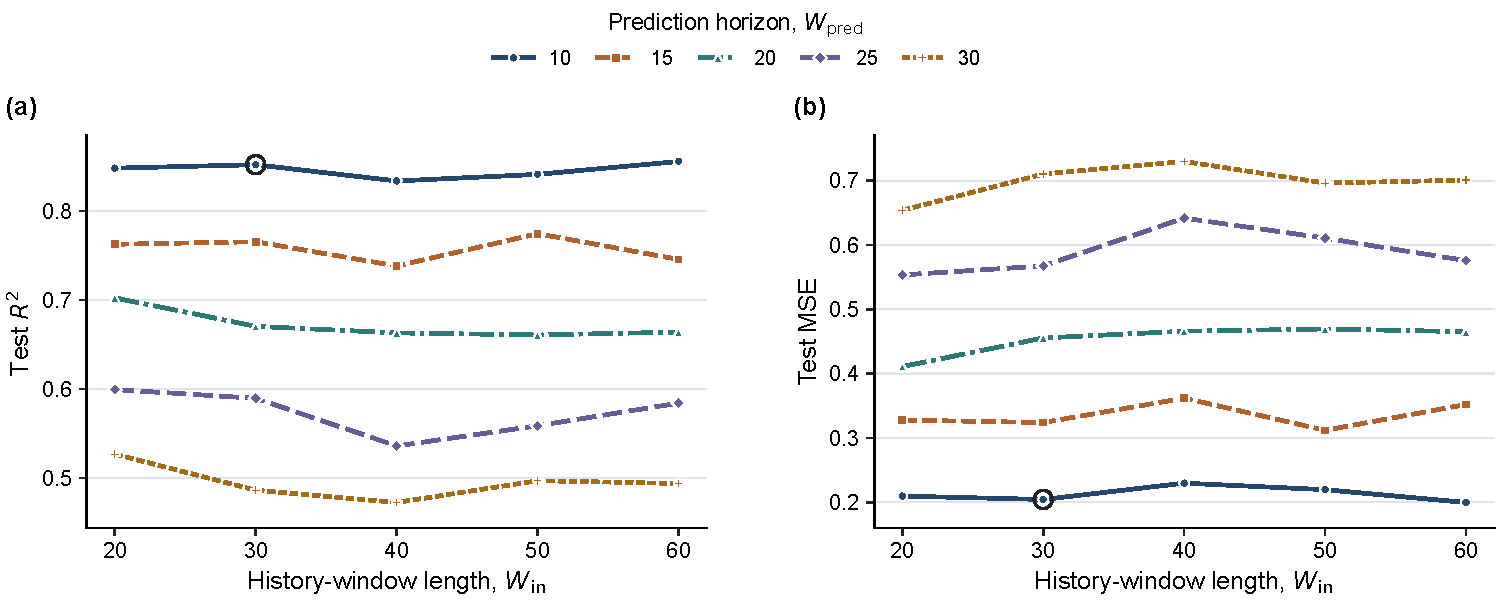
\includegraphics[width=.96\linewidth]{figs/window_sensitivity_publication.pdf}
	\caption{\rev{Sensitivity of source-domain test performance to history-window length under different prediction horizons: (a) $R^2$ and (b) MSE. The outlined point denotes the retained $W_{\mathrm{in}}=30$, $W_{\mathrm{pred}}=10$ setting.}}
	\label{fig:window_sensitivity}
\end{figure}

The prediction results in the source domain are shown in Fig.~\ref{fig:lstm_results_in_source}. Using the archived LSTM checkpoint subsequently employed for direct source-to-target deployment and transfer learning, the digital twin achieves $R^2=0.8824$, MSE $=0.1826$, RMSE $=0.4273$, and MAPE $=0.724\%$ on the validation set. On the held-out test set, the corresponding values are $R^2=0.8591$, MSE $=0.1946$, RMSE $=0.4411$, and MAPE $=0.755\%$. Thus, Fig.~\ref{fig:lstm_results_in_source}, Table~\ref{tab:source_model_comparison}, and the source-reference curve in Fig.~\ref{fig:residual_distribution} now report the same archived LSTM checkpoint.

\begin{figure}[pos=H]
	\centering
	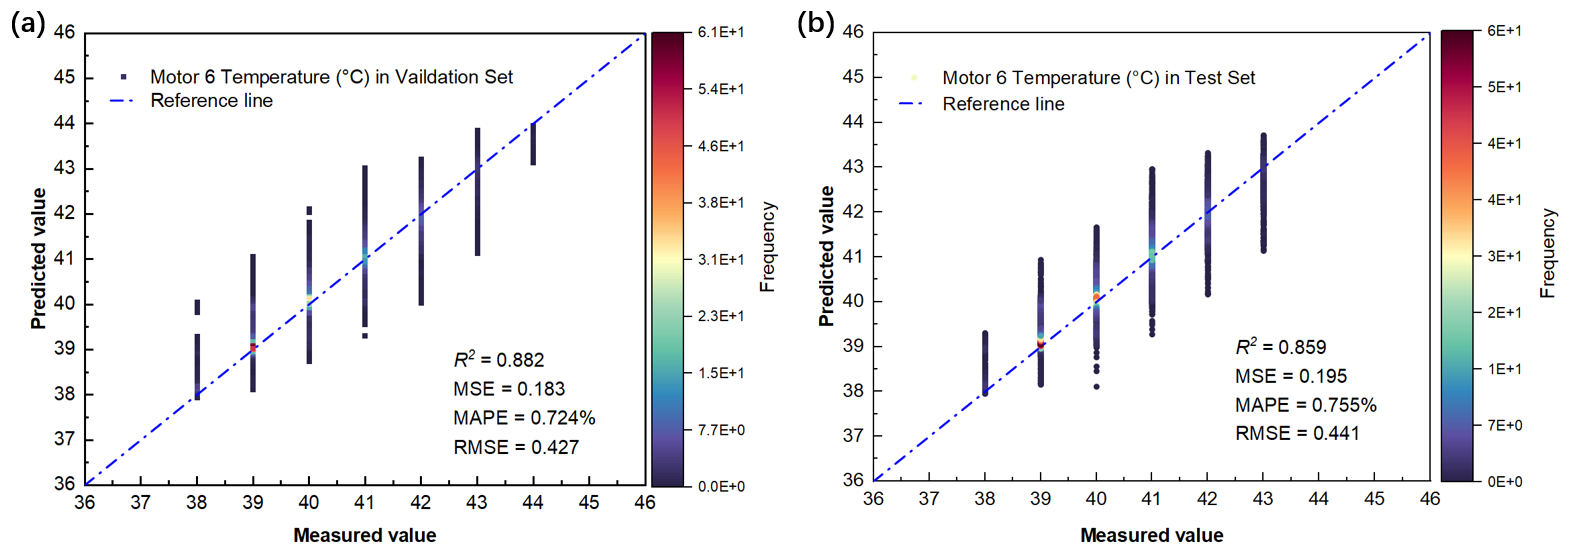
\includegraphics[width=1\linewidth]{figs/lstm_results_in_source.png}
	\caption{Prediction performance of the LSTM-based digital twin in the source domain. (a) Validation results. (b) Test results.}
	\label{fig:lstm_results_in_source}
\end{figure}

\subsubsection{Updating the digital twin through transfer learning}


On the target robot operating under degraded conditions, a series of training scenarios were constructed to systematically evaluate the adaptability of the source-domain digital twin and the effectiveness of different updating strategies, as summarized in Table~\ref{tab:tgt_data_scaling}. In all experiments, the target-domain test set was kept fixed with 1,521 samples, while the number of target-domain training samples used for model updating was gradually increased from 12.5\% (1,521 samples) to 100\% (12,441 samples). This experimental setting ensures a fair comparison of updating performance under different target-domain data availability, while eliminating the influence of variations in the test set.

\begin{table}[pos=H]
	\centering
	\caption{Training configurations in the target domain (after sample construction). Test sets are fixed.}
	\label{tab:tgt_data_scaling}
	\color{revisionred}
	\begin{tabular}{ccc}
		\toprule
		\textbf{Scenario} & \textbf{Usable Training Samples} &
		\textbf{Test Samples}                                                         \\
		\midrule
		1                 & 1,521 (12.5\%)                   & \multirow{8}{*}{1,521} \\
		2                 & 3,081 (25\%)                     &                        \\
		3                 & 4,641 (37.5\%)                   &                        \\
		4                 & 6,201 (50\%)                     &                        \\
		5                 & 7,761 (62.5\%)                   &                        \\
		6                 & 9,321 (75\%)                     &                        \\
		7                 & 10,881 (87.5\%)                  &                        \\
		8                 & 12,441 (100\%)                   &                        \\
		\bottomrule
	\end{tabular}
\end{table}


Based on this setup, a transfer-learning-based updating strategy is further evaluated, in which the target digital twin is initialized using the parameters learned from the source system and subsequently fine-tuned using healthy target-domain data. Following the digital twin updating mechanism introduced in Section~\ref{sec:3.3}, this transfer process is implemented via layer-wise fine-tuning of a three-layer LSTM predictor. The recurrent layers are indexed as layers~0,~1, and~2 from bottom to top. Different updating strategies are defined by selectively freezing lower layers while fine-tuning higher layers and the output fully connected (FC) layer, as follows:
\begin{itemize}
	\item Freeze LSTM layer~0; fine-tune layers~1--2 and the output FC layer;
	\item Freeze LSTM layers~0--1; fine-tune only layer~2 and the output FC layer;
	\item Freeze all LSTM layers (layers~0--2); fine-tune only the output FC layer;
	\item No layers frozen; fine-tune all LSTM layers (layers~0--2) and the output FC layer.
\end{itemize}

For experimental comparison, the source-trained digital twin is first directly deployed to the target domain as a \emph{direct generalization} baseline. In addition, a \emph{target-only learning} configuration is considered, where the model is trained from scratch using only target-domain data. Together with the layer-wise transfer updating strategies, these configurations enable a systematic comparison of digital twin modeling performance under degradation. The nominal temperature prediction results on the fault-free target-domain validation and test sets are shown in Fig.~\ref{fig:freeze_test}.


\begin{figure}[pos=H]
	\centering
	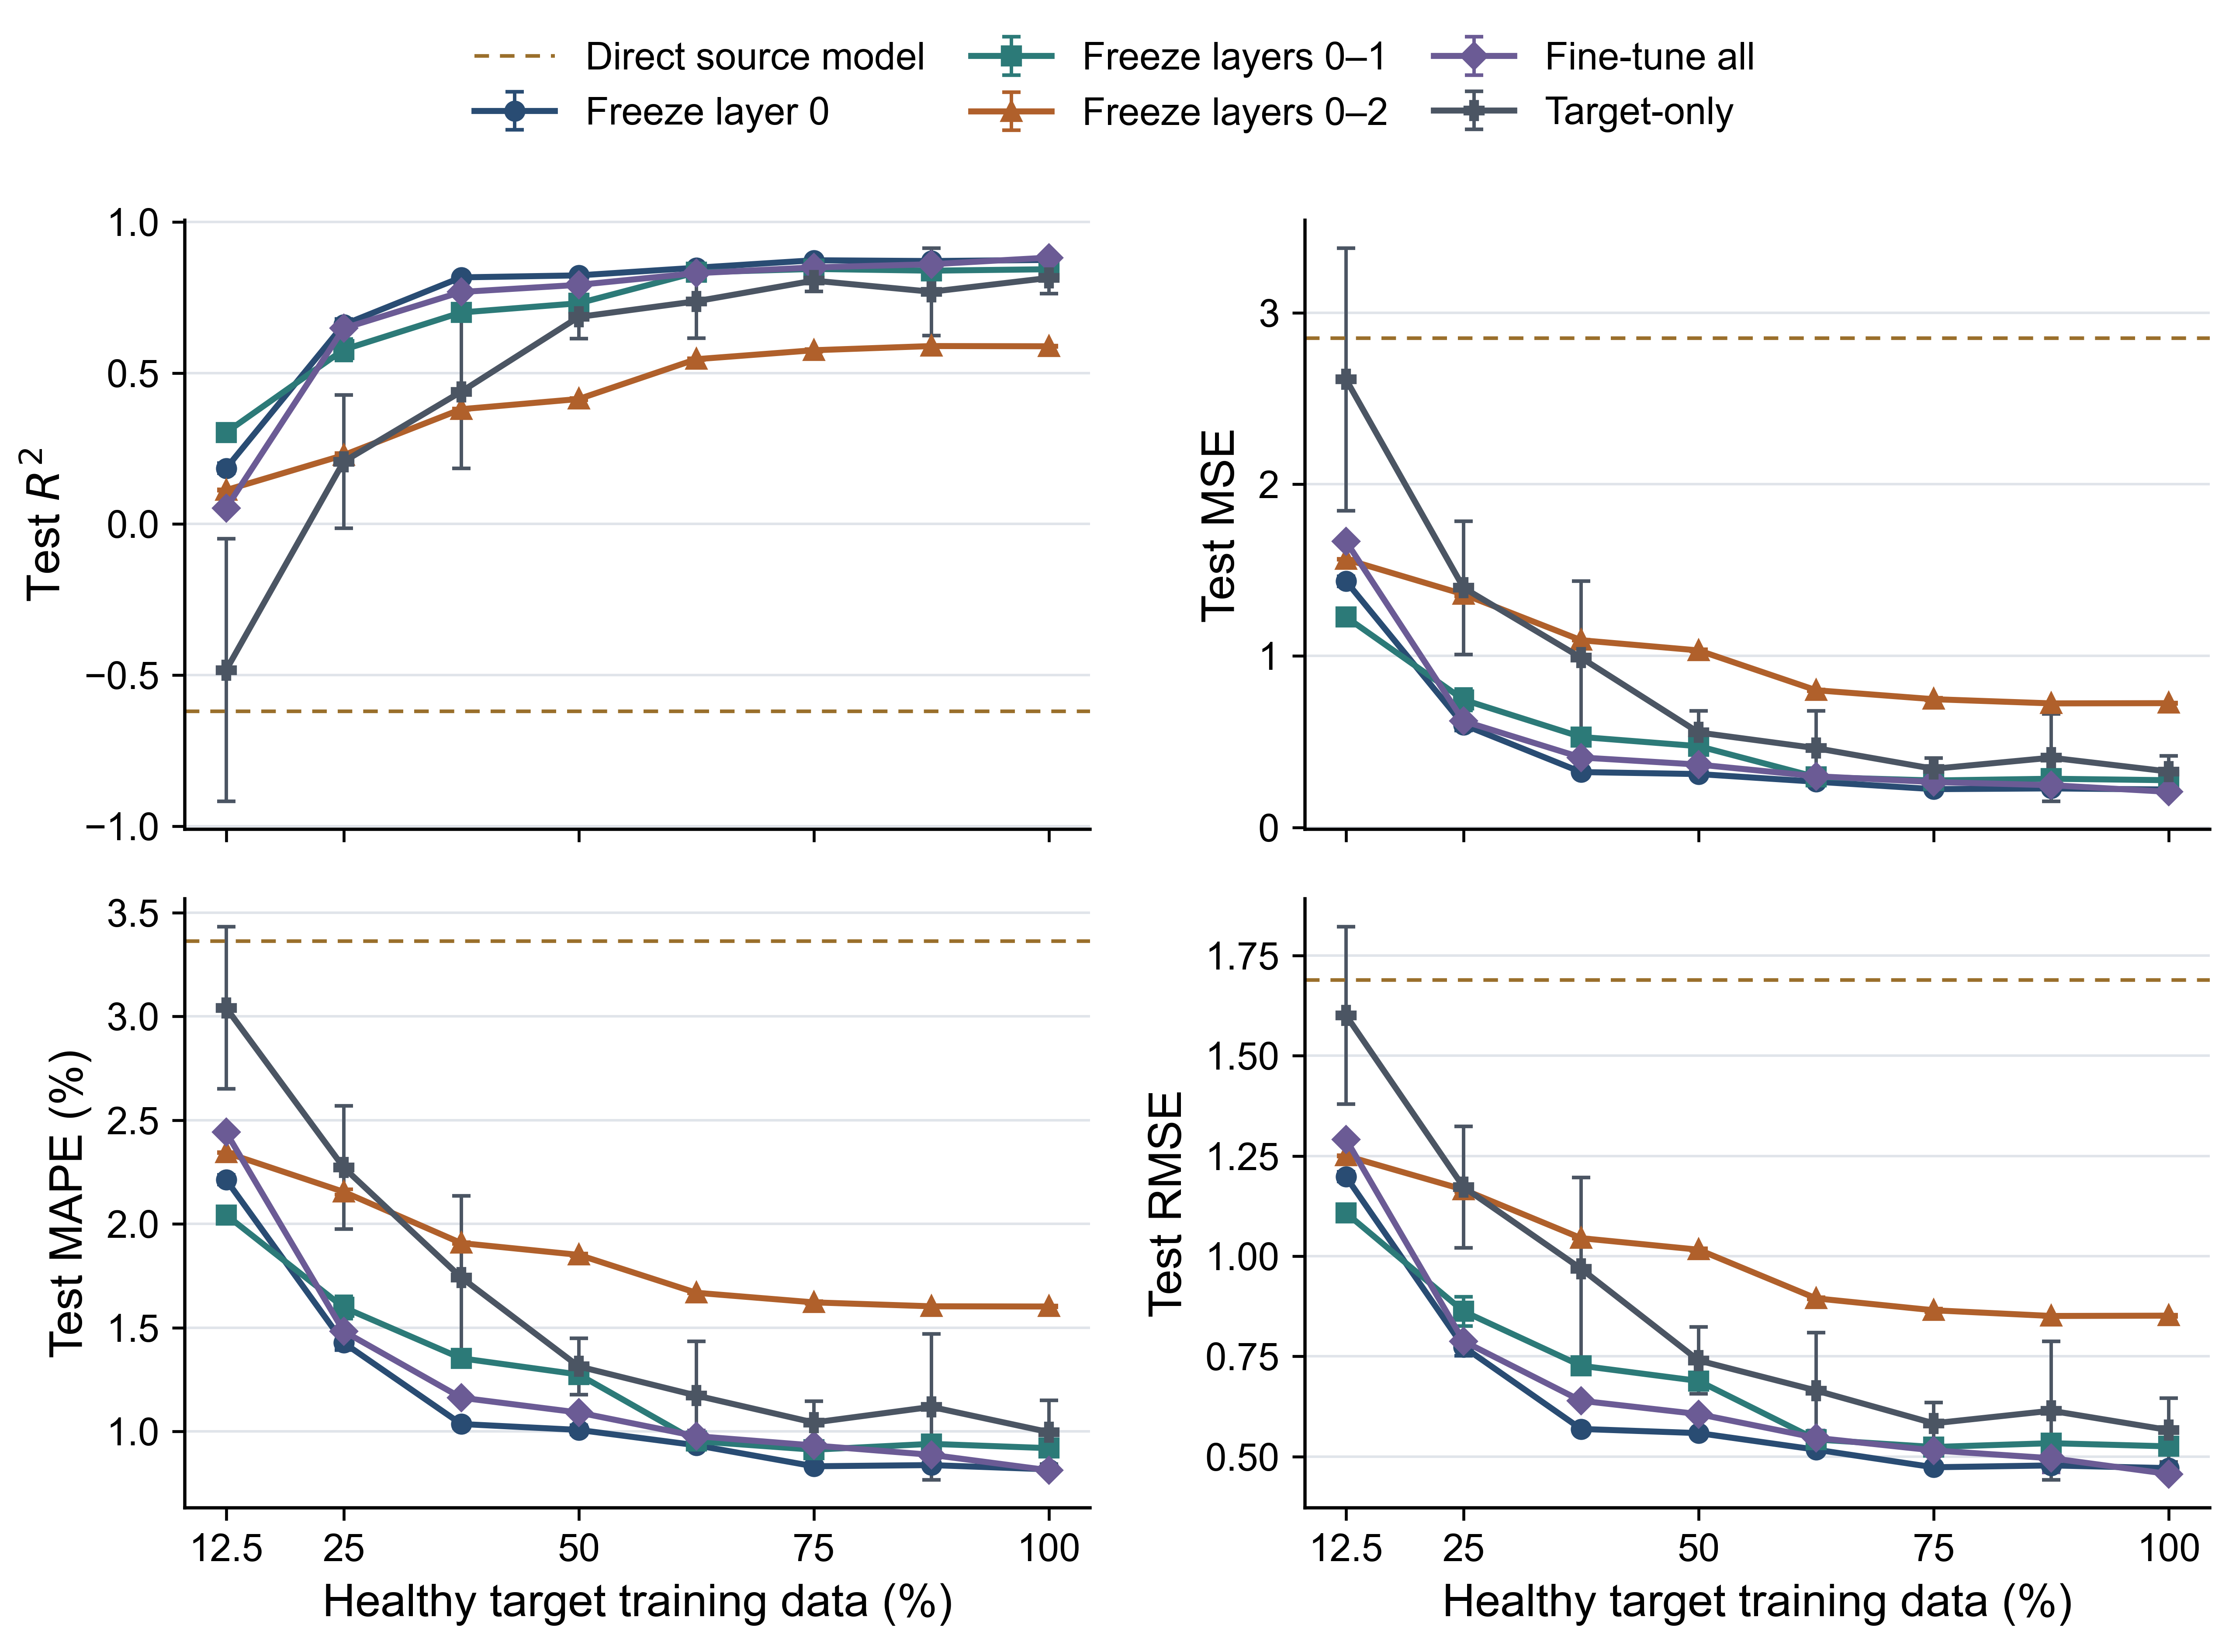
\includegraphics[width=1\linewidth]{figs/transfer_layers_test_publication.png}
	\caption{\rev{Nominal modeling performance on the target test set $\mathcal{D}_{\text{tgt}}^{\text{test}}$ under different layer-freezing configurations. Curves show the mean and error bars show one sample standard deviation over five independent seeds.}}
	\label{fig:freeze_test}
\end{figure}


It can be observed that direct generalization performs poorly across all evaluation metrics, with \(R^2\) values close to zero or even negative, and substantially higher MSE, RMSE, and MAPE compared to the updated models. This indicates that the system dynamics learned from the source robot are no longer sufficient to accurately characterize the thermal behavior of the degraded target robot without updating, experimentally confirming the degradation-induced cross-domain failure of a static digital twin. In contrast, target-only learning exhibits gradual performance improvement as more target-domain training samples become available, but remains consistently inferior to the transfer-based updating methods over the entire range of sample ratios, particularly under limited data availability, highlighting the limited data efficiency of learning from scratch.

As the proportion of target-domain training data increases, all transfer-based updating strategies exhibit a consistent performance improvement trend. Specifically, when the training sample ratio reaches approximately 25\%--50\%, the predictive performance is substantially recovered, with \(R^2\) increasing rapidly to above 0.6, and RMSE and MAPE reduced by more than half compared to the direct generalization baseline. When the sample ratio further increases beyond 75\%, the performance gains gradually saturate and additional improvements become marginal. These results demonstrate that even a limited amount of target-domain data is sufficient to effectively mitigate degradation-induced modeling errors through digital twin updating, highlighting the strong data efficiency of the proposed framework in the target domain.

A further comparison among different layer-freezing configurations reveals that the choice of frozen layers has a significant impact on updating performance. Among all strategies, freezing only the lowest layer (\emph{Freeze layer~0}) achieves the best or near-optimal performance across almost all target-domain sample ratios. In the low-to-medium sample regime (12.5\%--50\%), this configuration consistently yields higher \(R^2\) values and lower MSE, RMSE, and MAPE than the other strategies, while maintaining stable performance as the sample size increases. In contrast, fully fine-tuning all network parameters tends to result in degraded or unstable performance when target-domain data are limited, and target-only learning fails to match the performance of transfer-based updating under the same data conditions. Based on these observations, \emph{Freeze layer~0} is adopted as the default updating strategy for all subsequent target-domain digital twin updating experiments.

\begin{revision}
	Here, the target-only baseline is trained from random initialization using only healthy target-domain data; it contains no source parameters and is therefore the ``no transfer learning'' condition in the component ablation. For the residual-alignment analysis in Fig.~\ref{fig:residual_distribution}, the pre-transfer baseline is the same archived source LSTM reported in Fig.~\ref{fig:lstm_results_in_source} and Table~\ref{tab:source_model_comparison}, deployed on the target test set without any target-domain parameter update. The post-transfer curve is generated from this checkpoint after freezing LSTM layer~0 and fine-tuning the remaining layers on 100\% of the designated healthy target training split, with validation-based early stopping. The direct-generalization value in Figs.~\ref{fig:freeze_test} and~\ref{fig:residual_distribution} is identical, and the two target curves in Fig.~\ref{fig:residual_distribution} use the same 1,521 test windows and differ only by transfer adaptation. Direct source-to-target deployment yields MSE $=2.8525$ and $R^2=-0.6200$, whereas transfer learning reduces the MSE to $0.2170$ and raises $R^2$ to $0.8768$. Moreover, the Wasserstein distance between the target and source residual distributions decreases from $1.588$ to $0.157$, and the Kolmogorov--Smirnov statistic decreases from $0.820$ to $0.221$. These results show that transfer learning substantially reduces the prediction error toward the source reference and therefore provide empirical support, rather than a universal guarantee, for reusing the source-calibrated residual threshold under the sensing, preprocessing, and operating conditions stated in Section~\ref{sec:4.3}. The target-only results remain in the ablation comparison because they answer a different question: whether transferred initialization outperforms learning solely from target-domain data.
\end{revision}

\begin{figure}[pos=H]
	\centering
	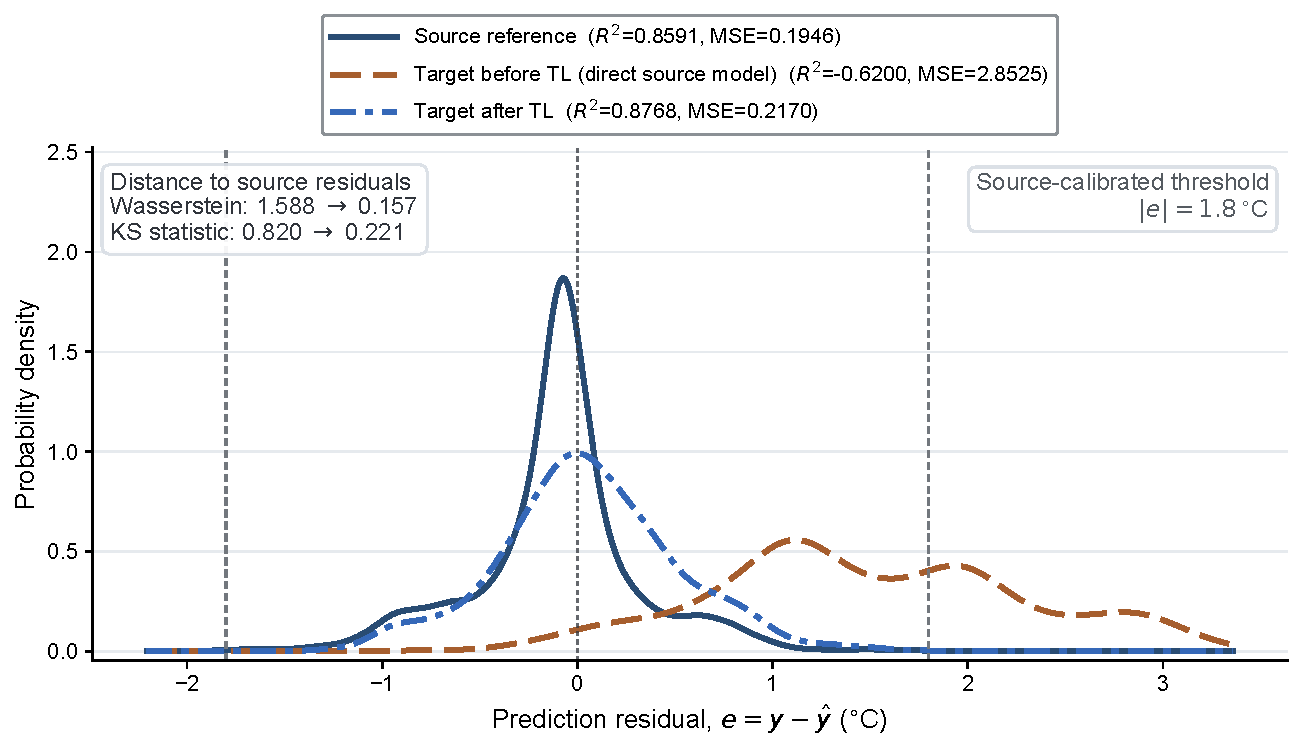
\includegraphics[width=.98\linewidth]{figs/residual_alignment_publication.pdf}
	\caption{\rev{Controlled residual-density comparison for the original transfer experiment underlying Fig.~\ref{fig:freeze_test}. The solid blue curve shows source-domain residuals; the red dashed curve shows the baseline obtained by applying the source-trained LSTM directly to the target test set; and the blue dashed curve shows target-domain residuals after transfer learning. Both target curves use the identical 1,521 test windows. The vertical dashed lines indicate the source-calibrated decision boundary $|e|=1.8\,^{\circ}$C.}}
	\label{fig:residual_distribution}
\end{figure}




\subsection{Residual-based fault detection performance}\label{sec:6.2}

\subsubsection{Threshold calibration}\label{sec:6.2.1}

This subsection addresses threshold calibration for the residual-based fault detection framework introduced in Section~\ref{sec:4}. Under rolling-horizon operation, the digital twin predicts motor temperature using healthy operational data, and fault detection is performed by comparing prediction residuals against a decision threshold. All experiments employ digital twins trained exclusively with healthy data as described in Section~\ref{sec:3.3}.

Motor~6 temperature is selected as the monitored variable. The point-wise residual $\epsilon(t)$ is computed according to Eq.~\eqref{eq:residual_definition}. To prevent information leakage, the residual threshold $\tau_{\mathrm{res}}$ is calibrated solely on the fault-injected source validation set $\mathcal{D}_{\text{src}}^{\text{val-fault}}$. \rev{All source fault subsets are transformed using the feature and target scalers saved with the trained LSTM checkpoint; the scalers are not refitted during threshold calibration or testing.}

\rev{A grid search is conducted over $\tau_{\mathrm{res}}\in[0,6]$ with step size 0.1, and the optimal threshold is selected by maximizing the F1-score (Eq.~\eqref{eq:threshold_optimization}). Figure~\ref{fig:threshold_opt} presents the resulting F1-score curve. A clear unimodal trend is observed, with the maximum F1-score of 0.8949 achieved at $\tau_{\mathrm{res}}=1.8$ when PROF is enabled. Smaller thresholds increase false positives due to noise sensitivity, whereas larger thresholds suppress informative residual deviations and increase missed detections.} \rev{Accordingly, $\tau_{\mathrm{res}}=1.8$ is fixed for all subsequent experiments on both source and target systems without re-calibration. This choice explicitly uses labeled injected faults in the source validation set. The deployment advantage is narrower: no target-domain fault labels or deliberate target-robot fault experiments are required. Cross-domain reuse is supported by the identical sensing and preprocessing pipeline and by the transfer-induced residual alignment in Fig.~\ref{fig:residual_distribution}, but is not claimed outside those conditions. It should be noted that in this paper, we calibrate the threshold only on the source domain validation data and directly use it on the target domain. This direct application works as long as the distributions of the residual errors between model predictions and observations are sufficiently similar in the source and target domains.
This condition may hold after transfer learning when the residual distributions of the two domains become sufficiently aligned.}

\begin{figure}[pos=H]
	\centering
	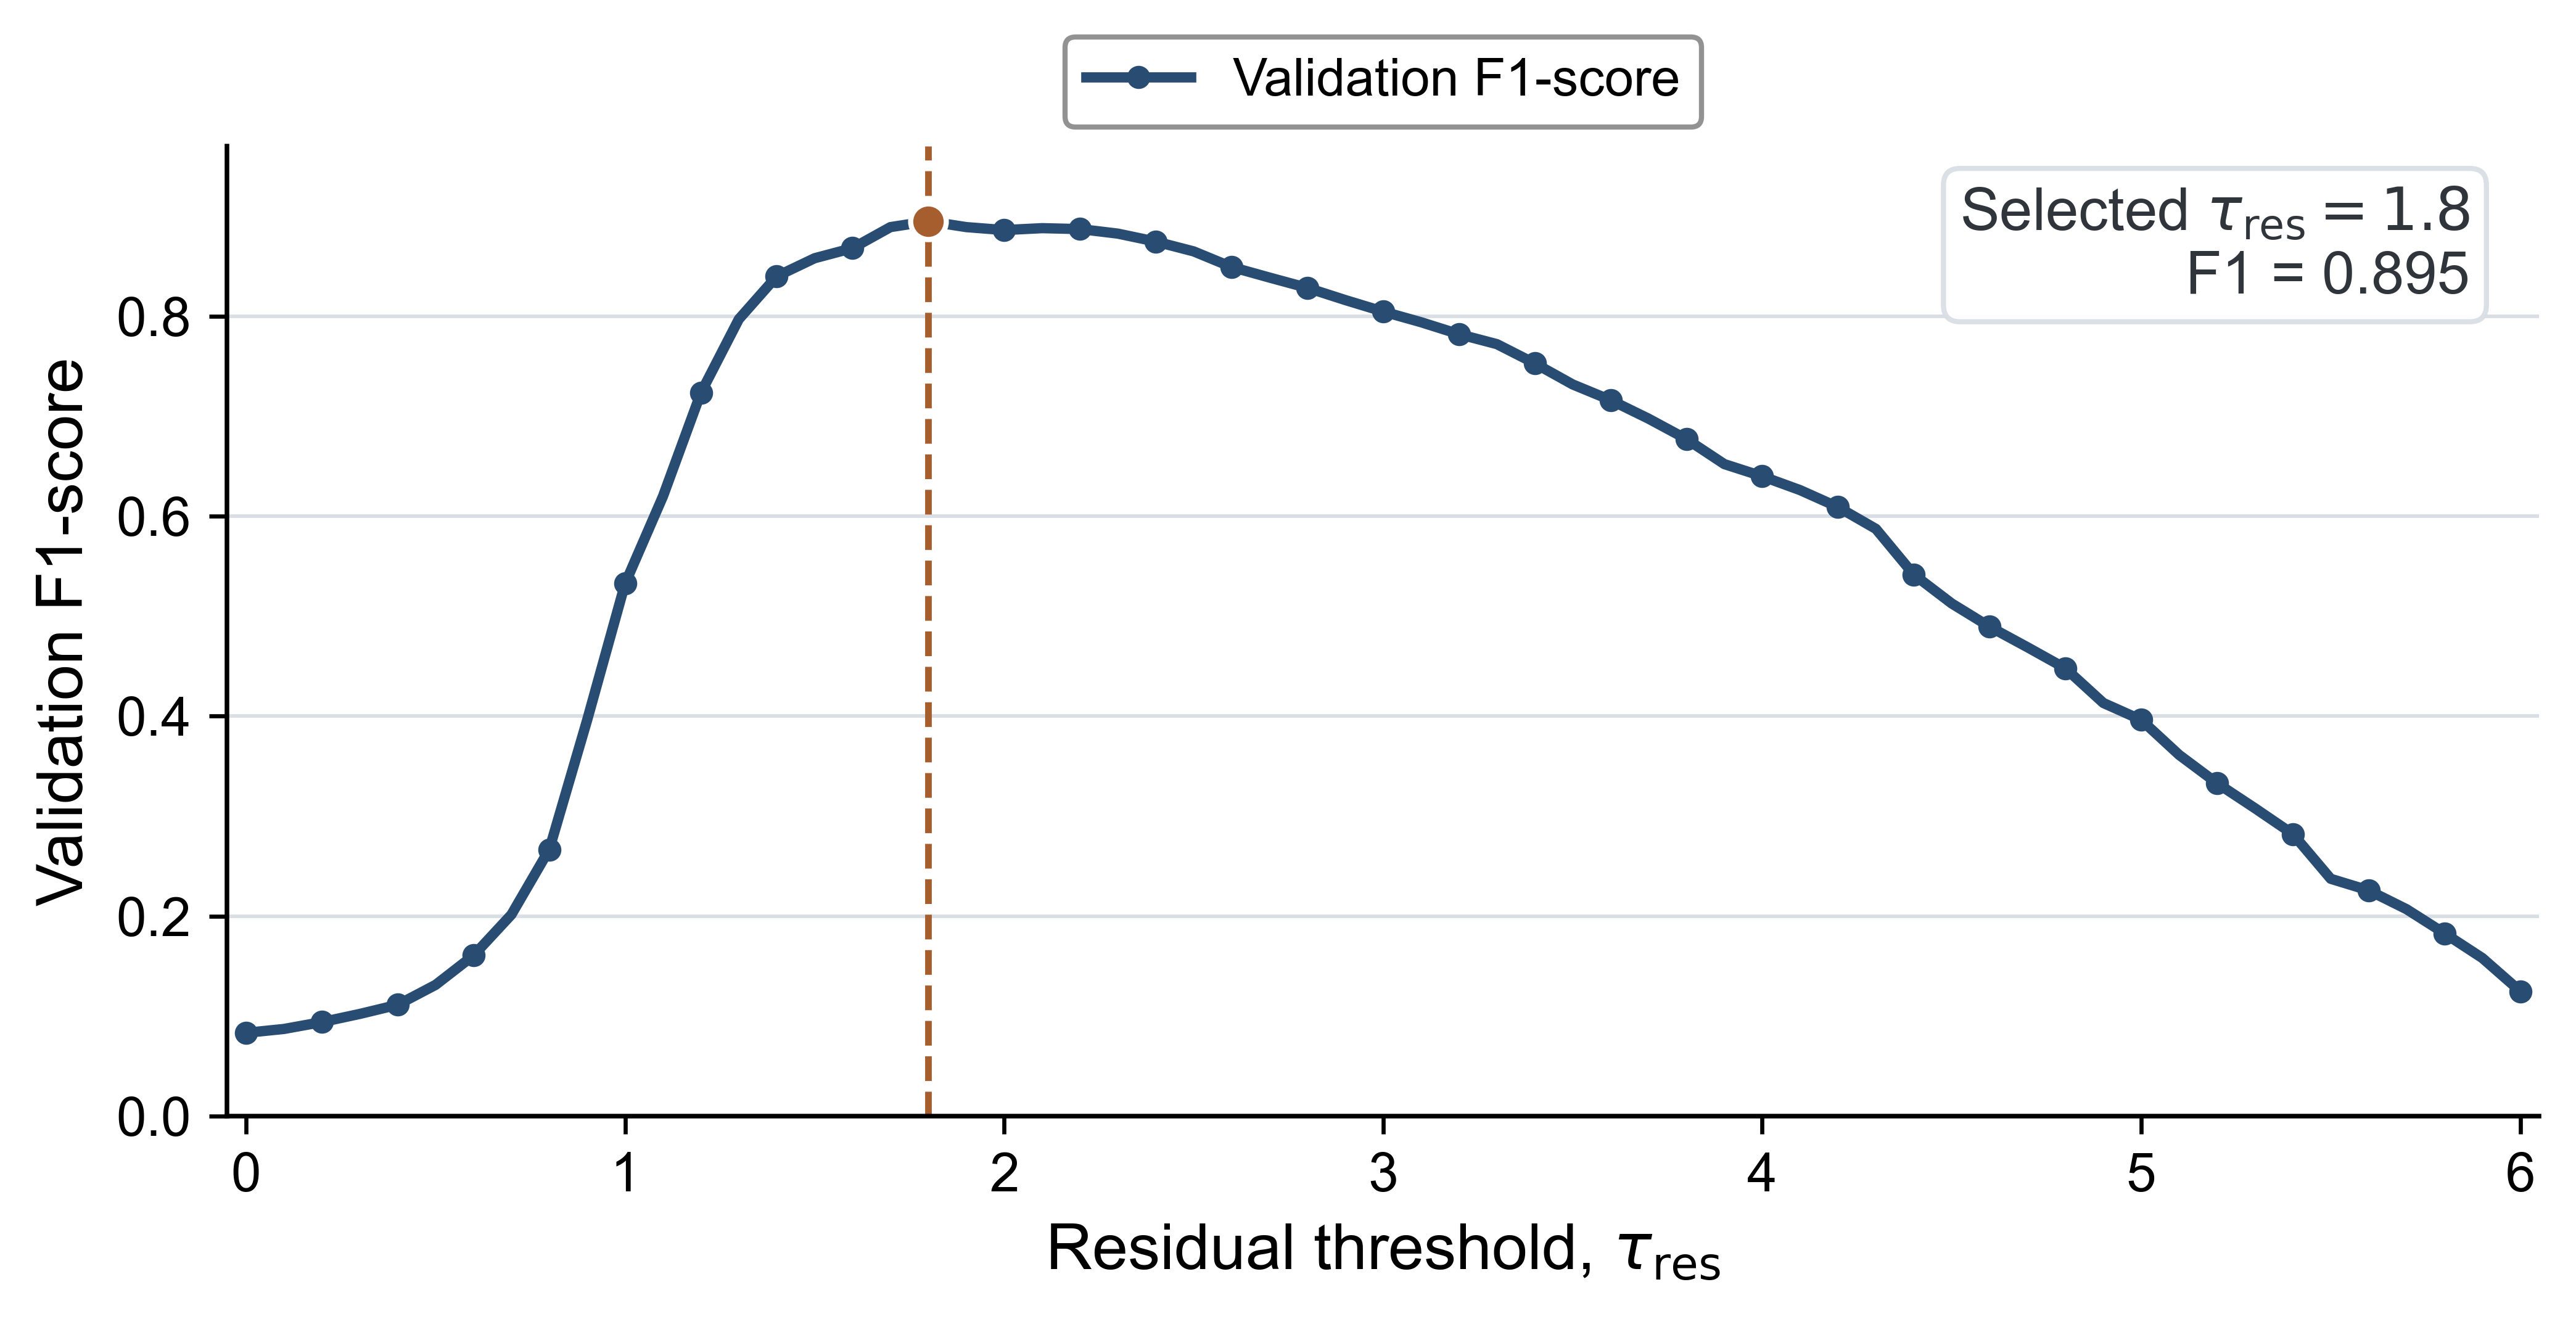
\includegraphics[width=.78\linewidth]{figs/threshold_opt_publication.png}
	\caption{\rev{F1-score versus residual threshold on the fault-injected source validation set $\mathcal{D}_{\text{src}}^{\text{val-fault}}$; the selected operating point is explicitly identified.}}
	\label{fig:threshold_opt}
\end{figure}

\subsubsection{Performance on the source domain}\label{sec:6.2.2}

\rev{With the threshold fixed at $\tau_{\text{res}} = 1.8$, residual-based fault detection is evaluated on the source system. The digital twin trained on healthy source data generates rolling-horizon predictions, and a binary decision is made based on the absolute residual at the final prediction step. A sample is classified as faulty when the residual exceeds $\tau_{\text{res}}$.}

\rev{Table~\ref{tab:source_fault_detection} summarizes the results on $\mathcal{D}_{\text{src}}^{\text{val-fault}}$ and $\mathcal{D}_{\text{src}}^{\text{test-fault}}$. On the validation set, the method achieves an accuracy of 0.9911 and an F1-score of 0.8949. On the unseen source-domain test set, it achieves an accuracy of 0.9904 and an F1-score of 0.8837. The small decrease on the test set indicates that the validation-selected threshold generalizes consistently to unseen source-domain trajectories.}

\rev{Although accuracy remains high due to the dominance of normal samples, recall and F1-score provide a more informative assessment of fault sensitivity. Precision remains above 0.91 on both subsets, demonstrating effective control of false alarms while retaining more than 0.84 recall on the unseen test trajectories.}

\begin{table}[pos=H]
	\centering
	\caption{Residual-based fault detection performance on the source domain}
	\label{tab:source_fault_detection}
	\renewcommand{\arraystretch}{1.2}
	\begin{tabular}{lcccc}
		\toprule
		\textbf{Dataset}                               & \textbf{Accuracy} & \textbf{Precision} & \textbf{Recall} & \textbf{F1-score} \\
		\midrule
		$\mathcal{D}_{\text{src}}^{\text{val-fault}}$  & 0.9911            & 0.9150             & 0.8757          & 0.8949            \\
		$\mathcal{D}_{\text{src}}^{\text{test-fault}}$ & 0.9904            & 0.9283             & 0.8432          & 0.8837            \\
		\bottomrule
	\end{tabular}
\end{table}



\subsubsection{Impact of transfer learning on target-domain detection}\label{sec:6.2.3}

\rev{The source-calibrated threshold $\tau_{\text{res}} = 1.8$ is directly applied to the target system without re-optimization.} For each target training ratio in Table~\ref{tab:tgt_data_scaling}, two digital twins are constructed:
(i) a transfer-based model initialized from source parameters and fine-tuned with healthy target data, and
(ii) a target-only model trained from scratch.
In both cases, fault detection follows the same residual construction and rolling-horizon scheme.

\rev{Figure~\ref{fig:transfer_target_results} presents detection performance on the target fault test set $\mathcal{D}_{\text{tgt}}^{\text{test-fault}}$. At the smallest 12.5\% target-training ratio, the two approaches have nearly identical mean F1-scores (0.4433 for transfer learning and 0.4414 for target-only learning), but the transferred model has substantially lower variability across seeds. From 25\% onward, transfer learning provides substantially higher accuracy, precision, recall, and F1-score at all intermediate ratios. At the full-data endpoint, the transferred model retains higher accuracy, precision, and F1-score, whereas target-only learning has slightly higher recall. Overall, the results support faster and more stable adaptation once a minimal amount of verified healthy target data is available, without claiming uniform superiority in every individual metric.}

\begin{figure}[pos=htbp]
	\centering
	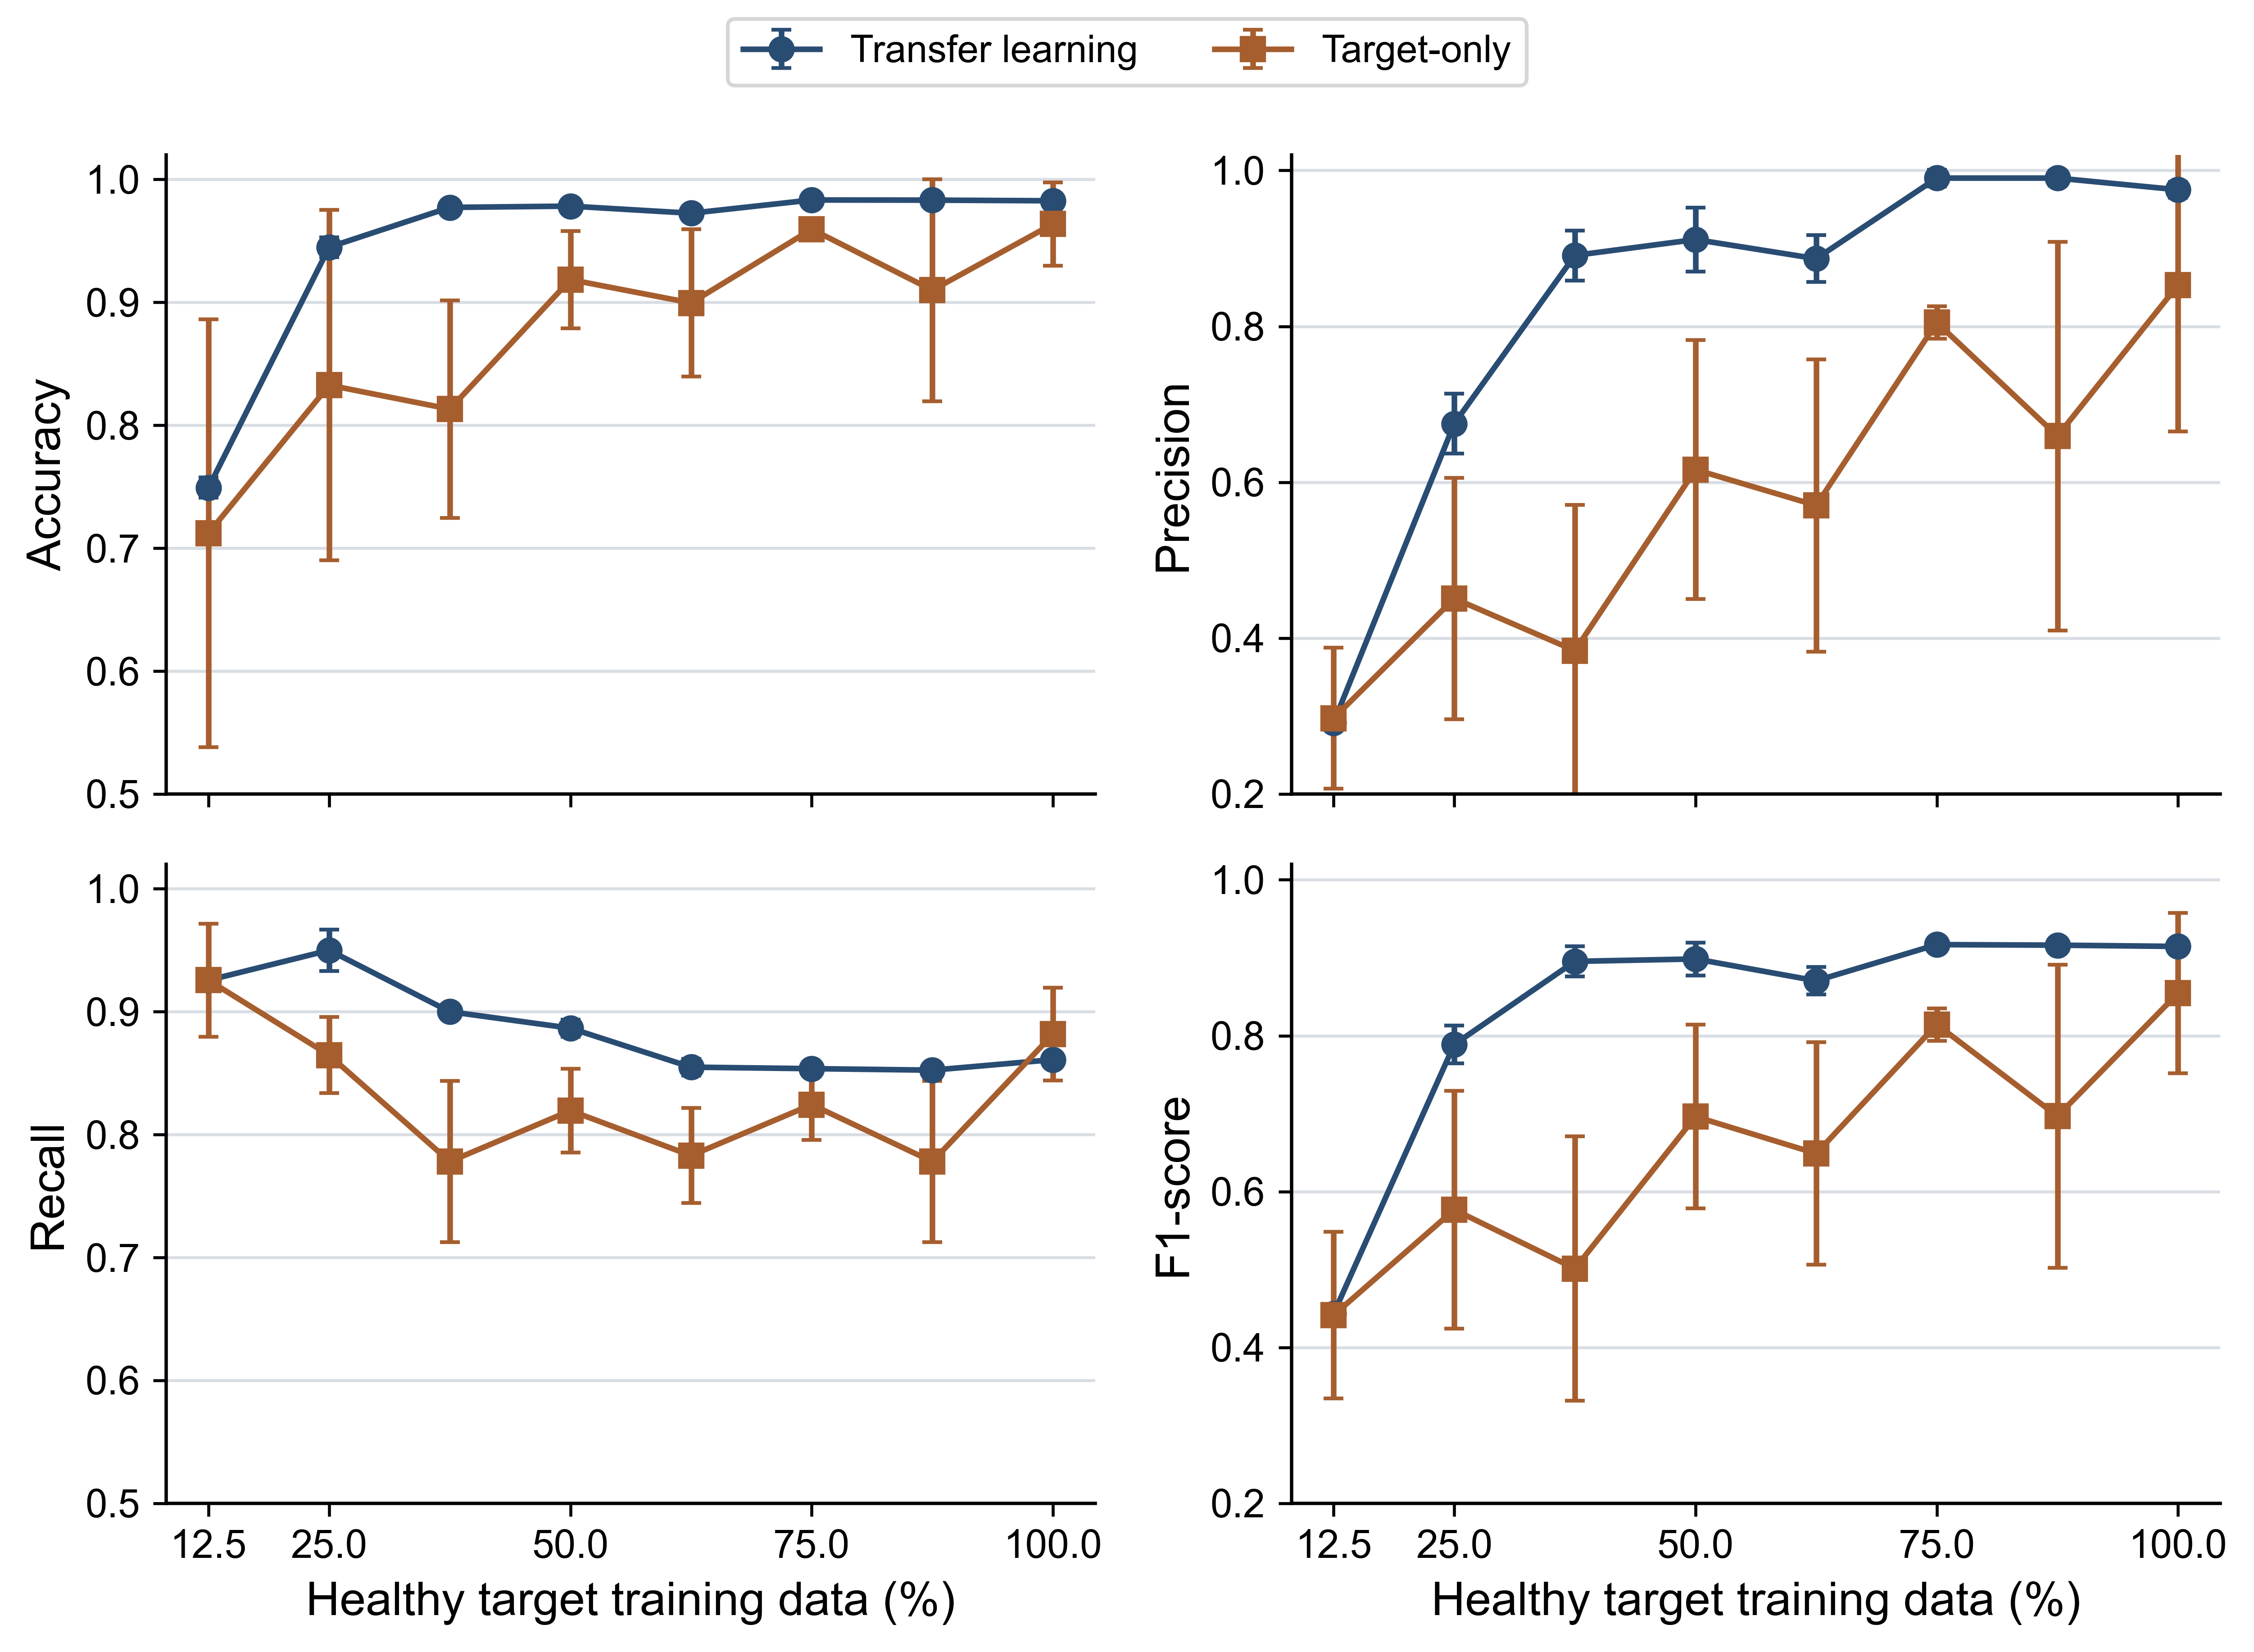
\includegraphics[width=.8\linewidth]{figs/test_transfer_publication.png}
	\caption{\rev{Fault detection performance on the fault-injected target test set $\mathcal{D}_{\text{tgt}}^{\text{test-fault}}$ under different proportions of healthy target training data. Curves show the mean and error bars show one sample standard deviation over five independent seeds.}}
	\label{fig:transfer_target_results}
\end{figure}



\subsubsection{Factorial ablation of transfer learning and PROF}\label{sec:6.2.4}

\begin{revision}
	Transfer learning (TL) and PROF are independently switched on and off in a controlled $2\times2$ factorial experiment on the same target-domain fault test set $\mathcal{D}_{\mathrm{tgt}}^{\mathrm{test-fault}}$. All configurations use the same DoE-acquired data, 100\% of the designated healthy target-domain training split $\mathcal{D}_{\mathrm{tgt}}^{\mathrm{train}}$, a 30-step input, a 10-step output, the fixed source-calibrated threshold $\tau_{\mathrm{res}}=1.8$, and identical test samples. ``No TL'' is the target-only LSTM trained from scratch; ``TL'' is the source-initialized LSTM with layer~0 frozen. Results are mean $\pm$ sample SD over seeds 42--46.
\end{revision}

\begin{table}[pos=H]
	\centering
	\color{revisionred}
	\caption{\color{revisionred}Controlled ablation of transfer learning and PROF on the target-domain fault test set.}
	\label{tab:tl_prof_ablation}
	\begin{tabular}{lcccc}
		\toprule
		Configuration   & Accuracy          & Precision         & Recall            & F1-score          \\
		\midrule
		No TL + No PROF & $0.9469\pm0.0057$ & $0.7640\pm0.0341$ & $0.7354\pm0.0196$ & $0.7493\pm0.0245$ \\
		No TL + PROF    & $0.9638\pm0.0339$ & $0.8531\pm0.1882$ & $0.8817\pm0.0377$ & $0.8546\pm0.1028$ \\
		TL + No PROF    & $0.9532\pm0.0009$ & $0.8240\pm0.0052$ & $0.7195\pm0.0043$ & $0.7682\pm0.0042$ \\
		TL + PROF       & $0.9826\pm0.0010$ & $0.9752\pm0.0101$ & $0.8610\pm0.0027$ & $0.9145\pm0.0045$ \\
		\bottomrule
	\end{tabular}
\end{table}

\begin{figure}[pos=H]
	\centering
	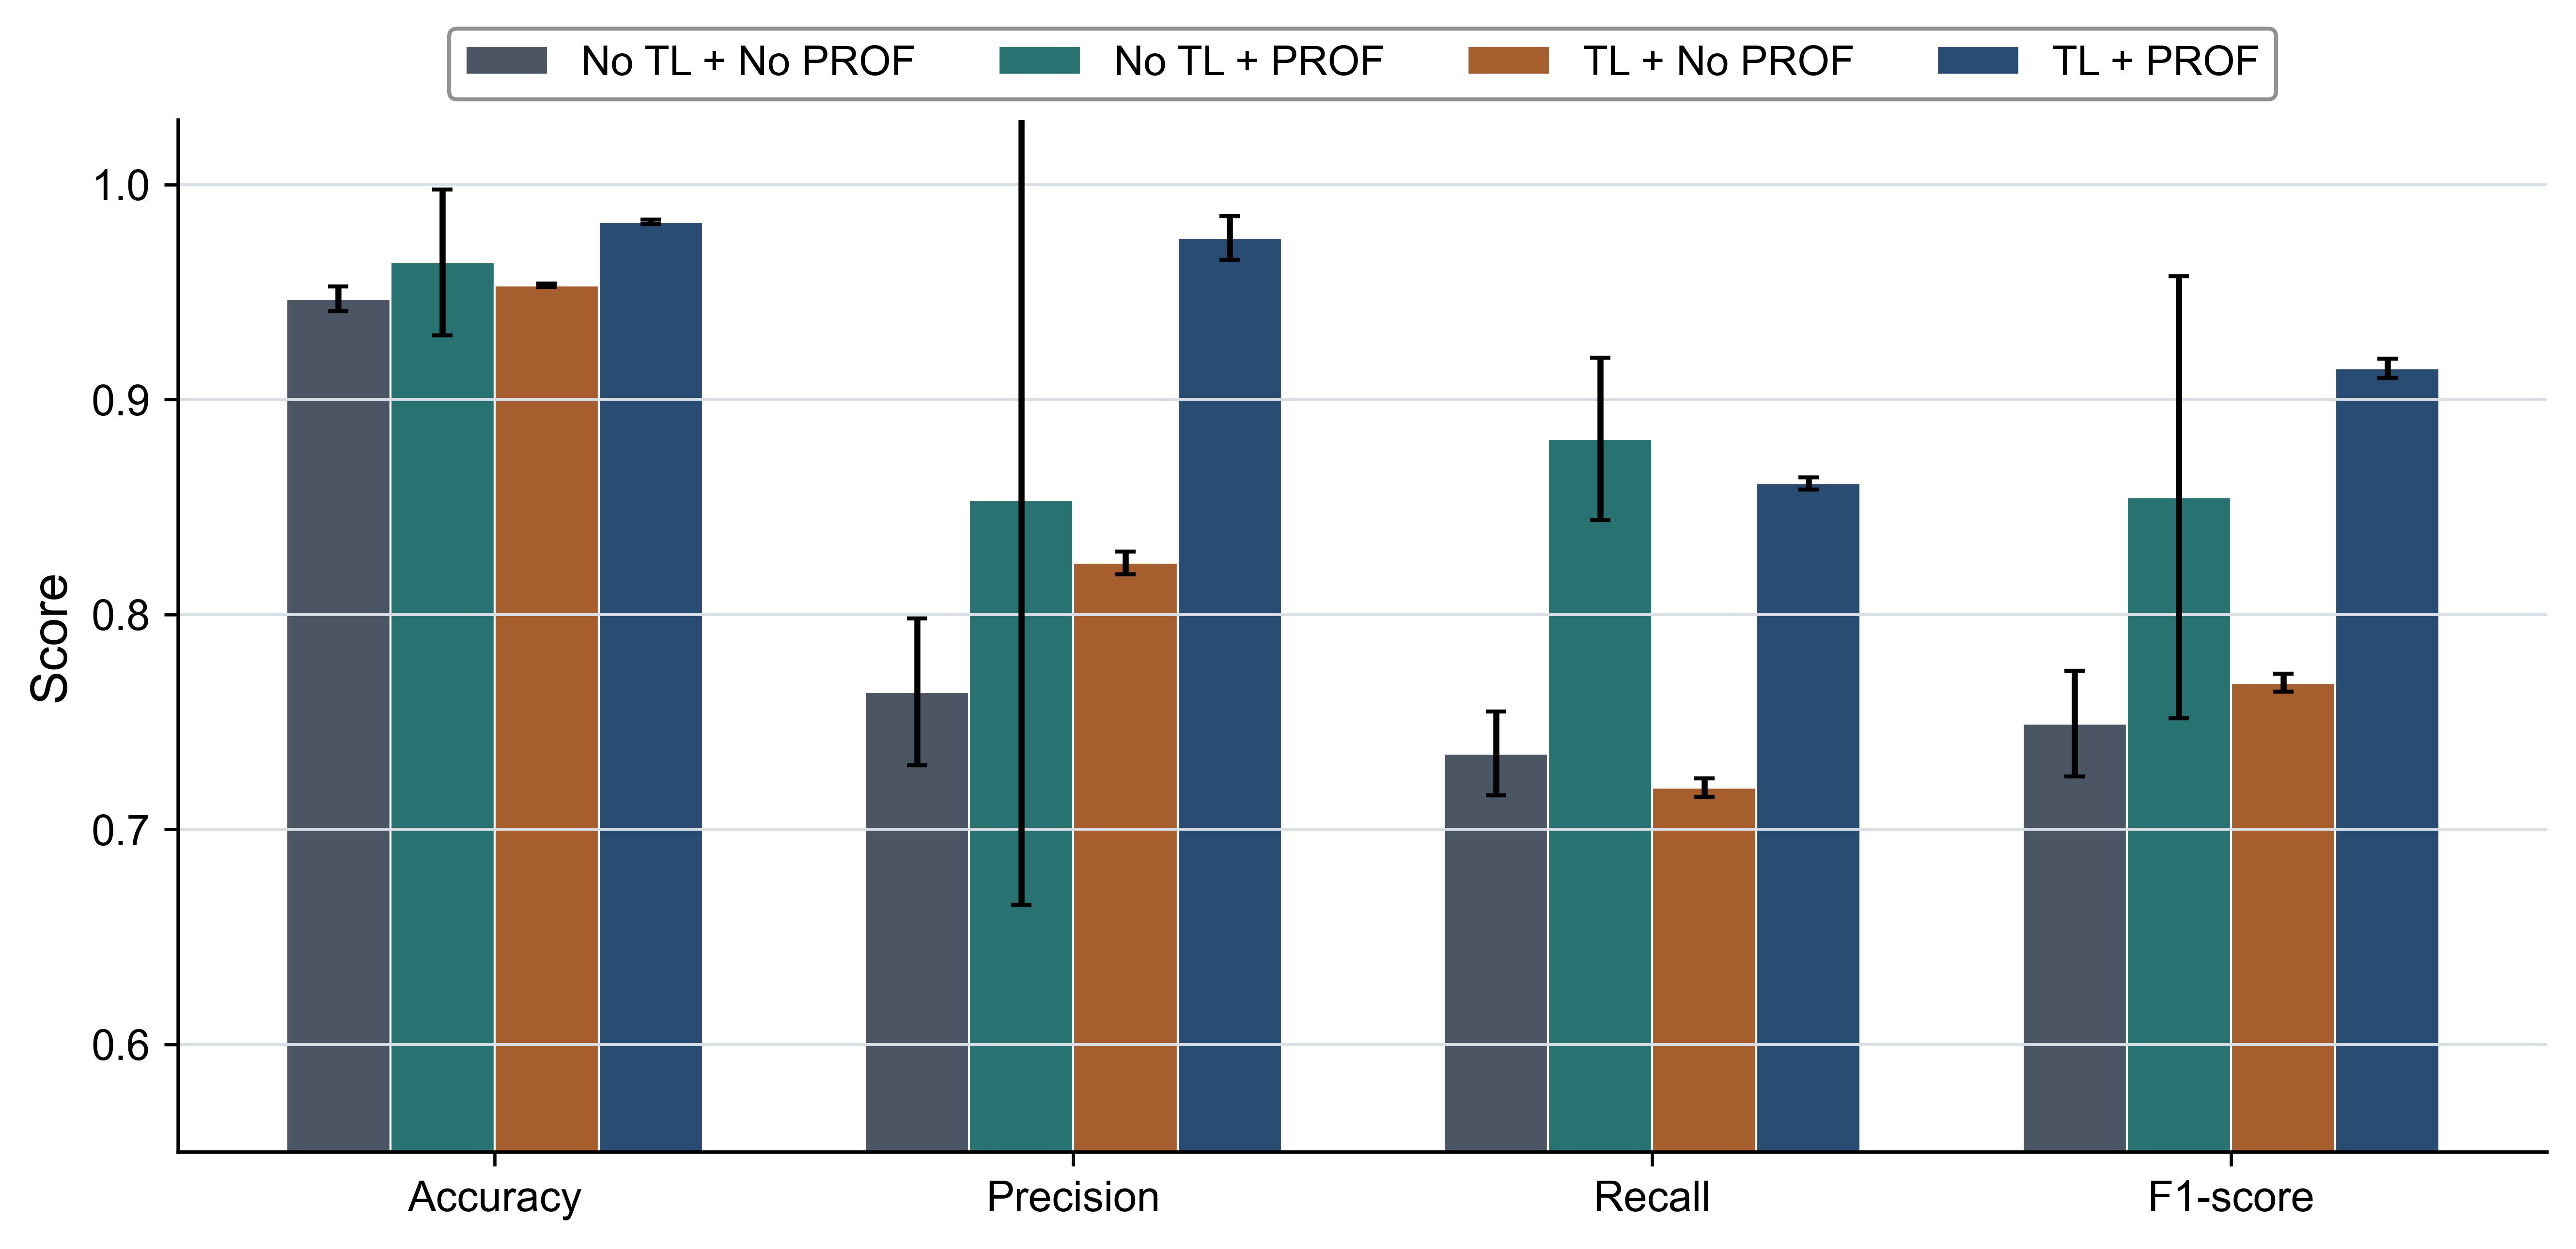
\includegraphics[width=.95\linewidth]{figs/ablation_tl_prof_publication.png}
	\caption{\rev{Fault-detection performance in the controlled TL$\times$PROF ablation. Bars and error bars denote the five-seed mean and sample standard deviation.}}
	\label{fig:prof_ablation}
\end{figure}

\begin{revision}
	The baseline without either component obtains an F1-score of $0.7493\pm0.0245$. PROF alone raises it to $0.8546\pm0.1028$, whereas TL alone raises it to $0.7682\pm0.0042$. Their combination gives the best overall accuracy ($0.9826\pm0.0010$), precision ($0.9752\pm0.0101$), and F1-score ($0.9145\pm0.0045$). Averaging over the paired factorial levels, the main F1-score effect is $+0.1258$ for PROF and $+0.0395$ for TL. PROF therefore provides the larger direct sensitivity gain, while TL reduces nominal cross-domain bias and markedly stabilizes the complete configuration: with PROF enabled, the F1 standard deviation falls from 0.1028 without TL to 0.0045 with TL.
\end{revision}


\subsection{Deployment-oriented computational efficiency}\label{sec:6.3}

\begin{revision}
	In this section, we report the training and inference latency of the different models used. Timing was measured on an NVIDIA RTX 1000 Ada Generation Laptop GPU. Inference measurements followed 100 warm-up iterations with explicit GPU synchronization; batch-1 latency used 500 repetitions and batch-64 latency used 200. Model-only timing isolates the forward pass, whereas end-to-end timing includes input transfer and output retrieval. Table~\ref{tab:deployment_timing} reports mean, median, and 95th-percentile latency. The selected LSTM requires a median 0.357~ms per end-to-end batch-1 query and 0.594~ms for batch 64. Its mean batch-1 end-to-end latency of 0.422~ms corresponds to approximately 2368 samples/s under this benchmark.
\end{revision}

\begin{table}[pos=H]
	\centering
	\color{revisionred}
	\caption{\color{revisionred}LSTM inference latency and transfer-learning fine-tuning time.}
	\label{tab:deployment_timing}
	\begin{tabular}{llccc}
		\toprule
		Metric      & Condition                    & Mean     & Median   & P95 or SD     \\
		\midrule
		Inference   & Batch 1, model only          & 0.414 ms & 0.460 ms & P95: 0.587 ms \\
		Inference   & Batch 1, end to end          & 0.422 ms & 0.357 ms & P95: 0.654 ms \\
		Inference   & Batch 64, end to end         & 0.624 ms & 0.594 ms & P95: 0.767 ms \\
		Fine-tuning & 100\% target training split, five seeds & 53.7 s   & --       & SD: 4.3 s     \\
		\bottomrule
	\end{tabular}
\end{table}

\begin{figure}[pos=H]
	\centering
	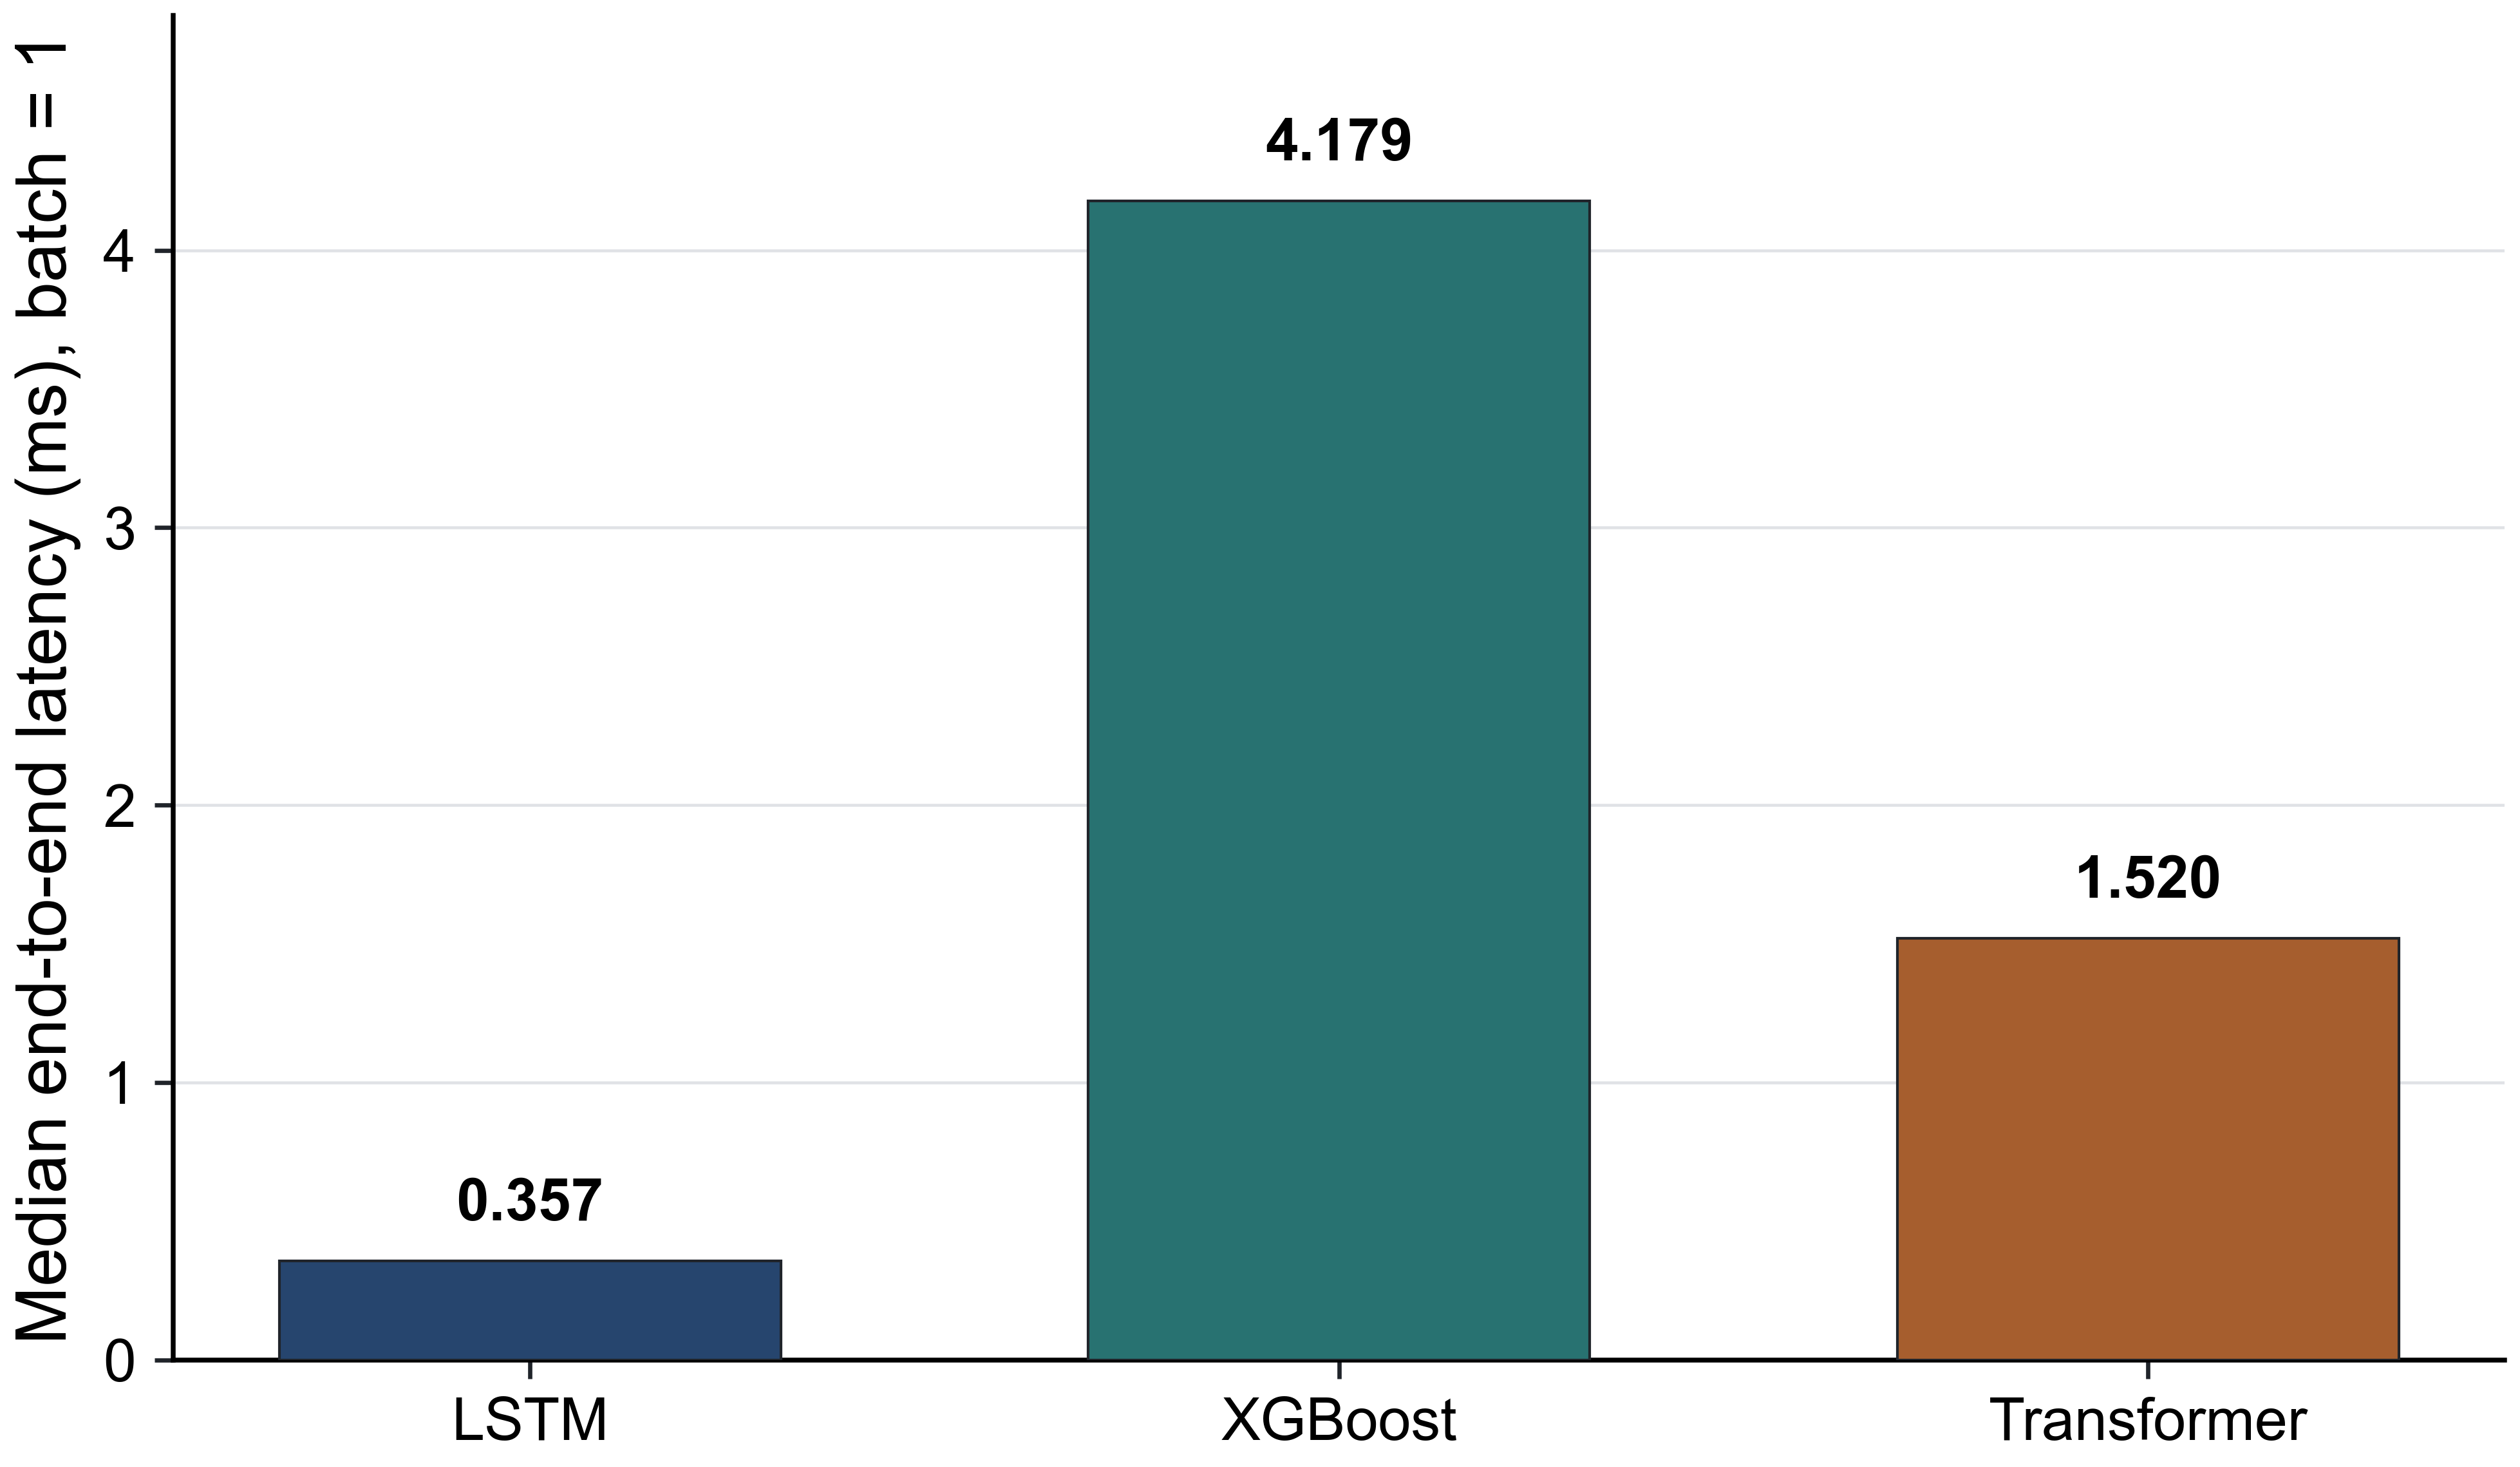
\includegraphics[width=.84\linewidth]{figs/source_model_latency_publication.png}
	\caption{\rev{Median end-to-end batch-1 inference latency during source-model screening.}}
	\label{fig:model_latency}
\end{figure}

\begin{revision}
	Figure~\ref{fig:model_latency} compares the same source-screening implementations: LSTM is fastest at 0.357~ms, compared with 1.520~ms for Transformer and 4.179~ms for XGBoost. Transfer-learning time is reported only for LSTM because Section~\ref{sec:6.1} selects the backbone before adaptation. Using 100\% of the designated verified healthy target-domain training split, freezing layer~0, batch size 64, learning rate $10^{-4}$, weight decay $10^{-4}$, at most 500 epochs, and patience 10, fine-tuning takes $53.7\pm4.3$~s over seeds 42--46 and stops after 77.2 epochs on average. Online inference is therefore comfortably sub-millisecond on the tested hardware, whereas model adaptation is positioned as an occasional low-frequency maintenance operation outside the real-time detection loop.
\end{revision}



\section{Conclusions}\label{sec:7}

\begin{revision}
	This study develops an integrated framework for data-driven digital-twin modeling and fault detection. Its main contribution is the integration of three building blocks: (i) a DoE-based data-generation procedure that uses Halton sampling to cover a bounded task-configuration envelope; (ii) a transfer-learning mechanism that adapts the digital twin to system evolution and cross-domain distribution shifts using verified healthy target-domain data; and (iii) a prediction-based recursive observation feedback (PROF) mechanism that prevents detected abnormal observations from contaminating subsequent rolling input windows. Together, these components support reliable nominal modeling and residual-based detection under model drift and fault-induced input contamination.

	The framework is validated on two physical robotic arms. The archived LSTM digital twin accurately reconstructs nominal motor-temperature behavior, achieving $R^2=0.8591$ and MAPE $=0.755\%$ on held-out source-domain test trajectories; it is retained because it offers competitive accuracy, the smallest model footprint, the lowest inference latency, and direct compatibility with parameter transfer. In the controlled residual-alignment experiment reported in Figs.~\ref{fig:freeze_test} and~\ref{fig:residual_distribution}, direct deployment of this source LSTM on the target test set gives MSE $=2.8525$ and $R^2=-0.6200$, whereas adaptation of the same checkpoint reduces MSE to $0.2170$ and raises $R^2$ to $0.8768$; the target-to-source Wasserstein residual distance correspondingly decreases from $1.588$ to $0.157$. This supports reuse of the source-calibrated threshold after healthy target-domain adaptation under matched sensing, preprocessing, and operating conditions, without requiring target-domain fault labels. A controlled $2\times2$ ablation shows that PROF provides the larger direct F1-score improvement ($+0.1258$), while transfer learning contributes a smaller but stabilizing effect (F1-score $+0.0395$, standard deviation reduced from $0.1028$ to $0.0045$ when PROF is enabled); the complete TL+PROF configuration achieves the best target-domain F1-score of $0.9145$. Timing experiments further confirm sub-millisecond online inference ($0.357$ ms median batch-1 latency) and target-domain fine-tuning in under one minute.

	This study has several limitations that point to future work. First, the residual threshold is calibrated on labeled fault-injected source-domain validation data; although no target-domain fault labels are required, the current procedure is not fully independent of labeled fault data, and a normal-data-only threshold based on an upper quantile or statistical confidence bound of healthy residuals is a natural extension. Second, the injected thermal faults follow a first-order lumped-parameter thermal model and represent progressive thermal anomalies rather than the full electromechanical signatures of real motor failures; validation on naturally occurring or safely reproduced physical faults would provide stronger evidence. Third, the verify-then-update policy assumes that gradual healthy drift requiring model adaptation can be distinguished from fault signals that must be excluded; fully automatic discrimination between the two is not addressed and remains an important direction for future work.
\end{revision}

%
% Declaration
%
\section*{Declaration of generative AI and AI-assisted technologies in the writing process}
\rev{During the preparation of this work, the author(s) used ChatGPT and GLM-5.2 to refine the language of the completed manuscript. After using this tool, the author(s) reviewed and edited the content as needed and take(s) full responsibility for the content of the published article.}


\section*{Declaration of Competing Interest}
The authors declare that they have no known competing financial interests or personal relationships that could have appeared to influence the work reported in this paper.


%% Loading bibliography style file%% Loading bibliography style file
% \bibliographystyle{cas-model2-names}
% \bibliographystyle{elsarticle-harv}
\bibliographystyle{elsarticle-num-names}


% Loading bibliography database% Loading bibliography database
\bibliography{cas-refs}




\end{document}
